\chapter{NNQS exploration}\label{nnqsresults}
In this chapter, we will explore the different architectures and training schemes that can be used for training the NNQS to solve QUBO problems. All experiments in this section were run on a subset of the full dataset with problem sizes of $10,25,50,75,200,250$ and $10$ problems for each problem type and size. The problem evaluation metrics are also calculated by considering the solutions from the different types of NNQS to be able to draw a clearer comparison between architectures and training schemes.

\section{Architectures and training algorithms}
We will utilize both the Restricted Boltzmann Machine (RBM) and the Multilayer Perceptron (MLP) in their performance as a NNQS. For a given input problem with $n$ variables, the RBM model will have $n$ visible nodes and $5n$ hidden nodes while the MLP will have $n$ input nodes, $1$ hidden layer of size $5n$ and $1$ positive real output node. The RBM uses the sigmoid function while the MLP uses the ReLU activation function. We use Gibbs sampling for the RBM and Metropolis-Hasting sampling for the MLP, both sampling methods are detailed in \autoref{samplingmethods}.

We will also compare 3 training algorithms for NNQS---progressive, direct, and continuous. The progressive training algorithm follows \autoref{alg:progressive}. In direct training, the normalized anneal fraction $s$ is held constant at $1$ for all epochs and follows \autoref{alg:direct}.  In continuous training, the NNQS is not trained to convergence but is trained for a single epoch while incrementing the normalized anneal fraction slowly and follows \autoref{alg:continuous}.

\begin{algorithm}
    \begin{algorithmic}
    \Require Problem Hamiltonian $\hat{H}_c$
    \Ensure Trained NNQS
    \State Initialize NNQS with random weights;
    \State Set $H \leftarrow B(1)\hat{H}_c$;
    \State Train NNQS on $H$ until convergence or until epoch limit of $1000$ is reached;
    \end{algorithmic}
    \caption{NNQS Direct Training}
    \label{alg:direct}
\end{algorithm}

\begin{algorithm}
    \begin{algorithmic}
    \Require Problem Hamiltonian $\hat{H}_c$
    \Ensure Trained NNQS
    \State Initialize NNQS with random weights;
    \For {$s \in [0.001, 1.0]$ step $0.001$}
    \State Set $H(s) \leftarrow A(s)\hat{H}_0 + B(s)\hat{H}_c$;
    \State Train NNQS on $H(s)$ for $1$ epoch;
    \EndFor
    \end{algorithmic}
    \caption{NNQS Continuous Training}
    \label{alg:continuous}
\end{algorithm}

Direct training serves as a baseline for directly training a neural network with the cost function as the problem Hamiltonian. Progressive training most closely resembles the quantum annealing process, where the system is kept at the ground state by training until convergence in each increment of $s$. Continuous training is a combination of the other two by slowly incrementing $s$ but never reaching convergence.

\section{Results and Discussion}
Performance is shown for each of the datasets, accompanied by error bars representing the unbiased standard error of the mean for each data point. Graphs with problem sizes on the x-axis are plotted with a log scale.

\subsection{NAE3SAT}

\begin{figure}[!htbp]
    \subfloat[Normalized energy]{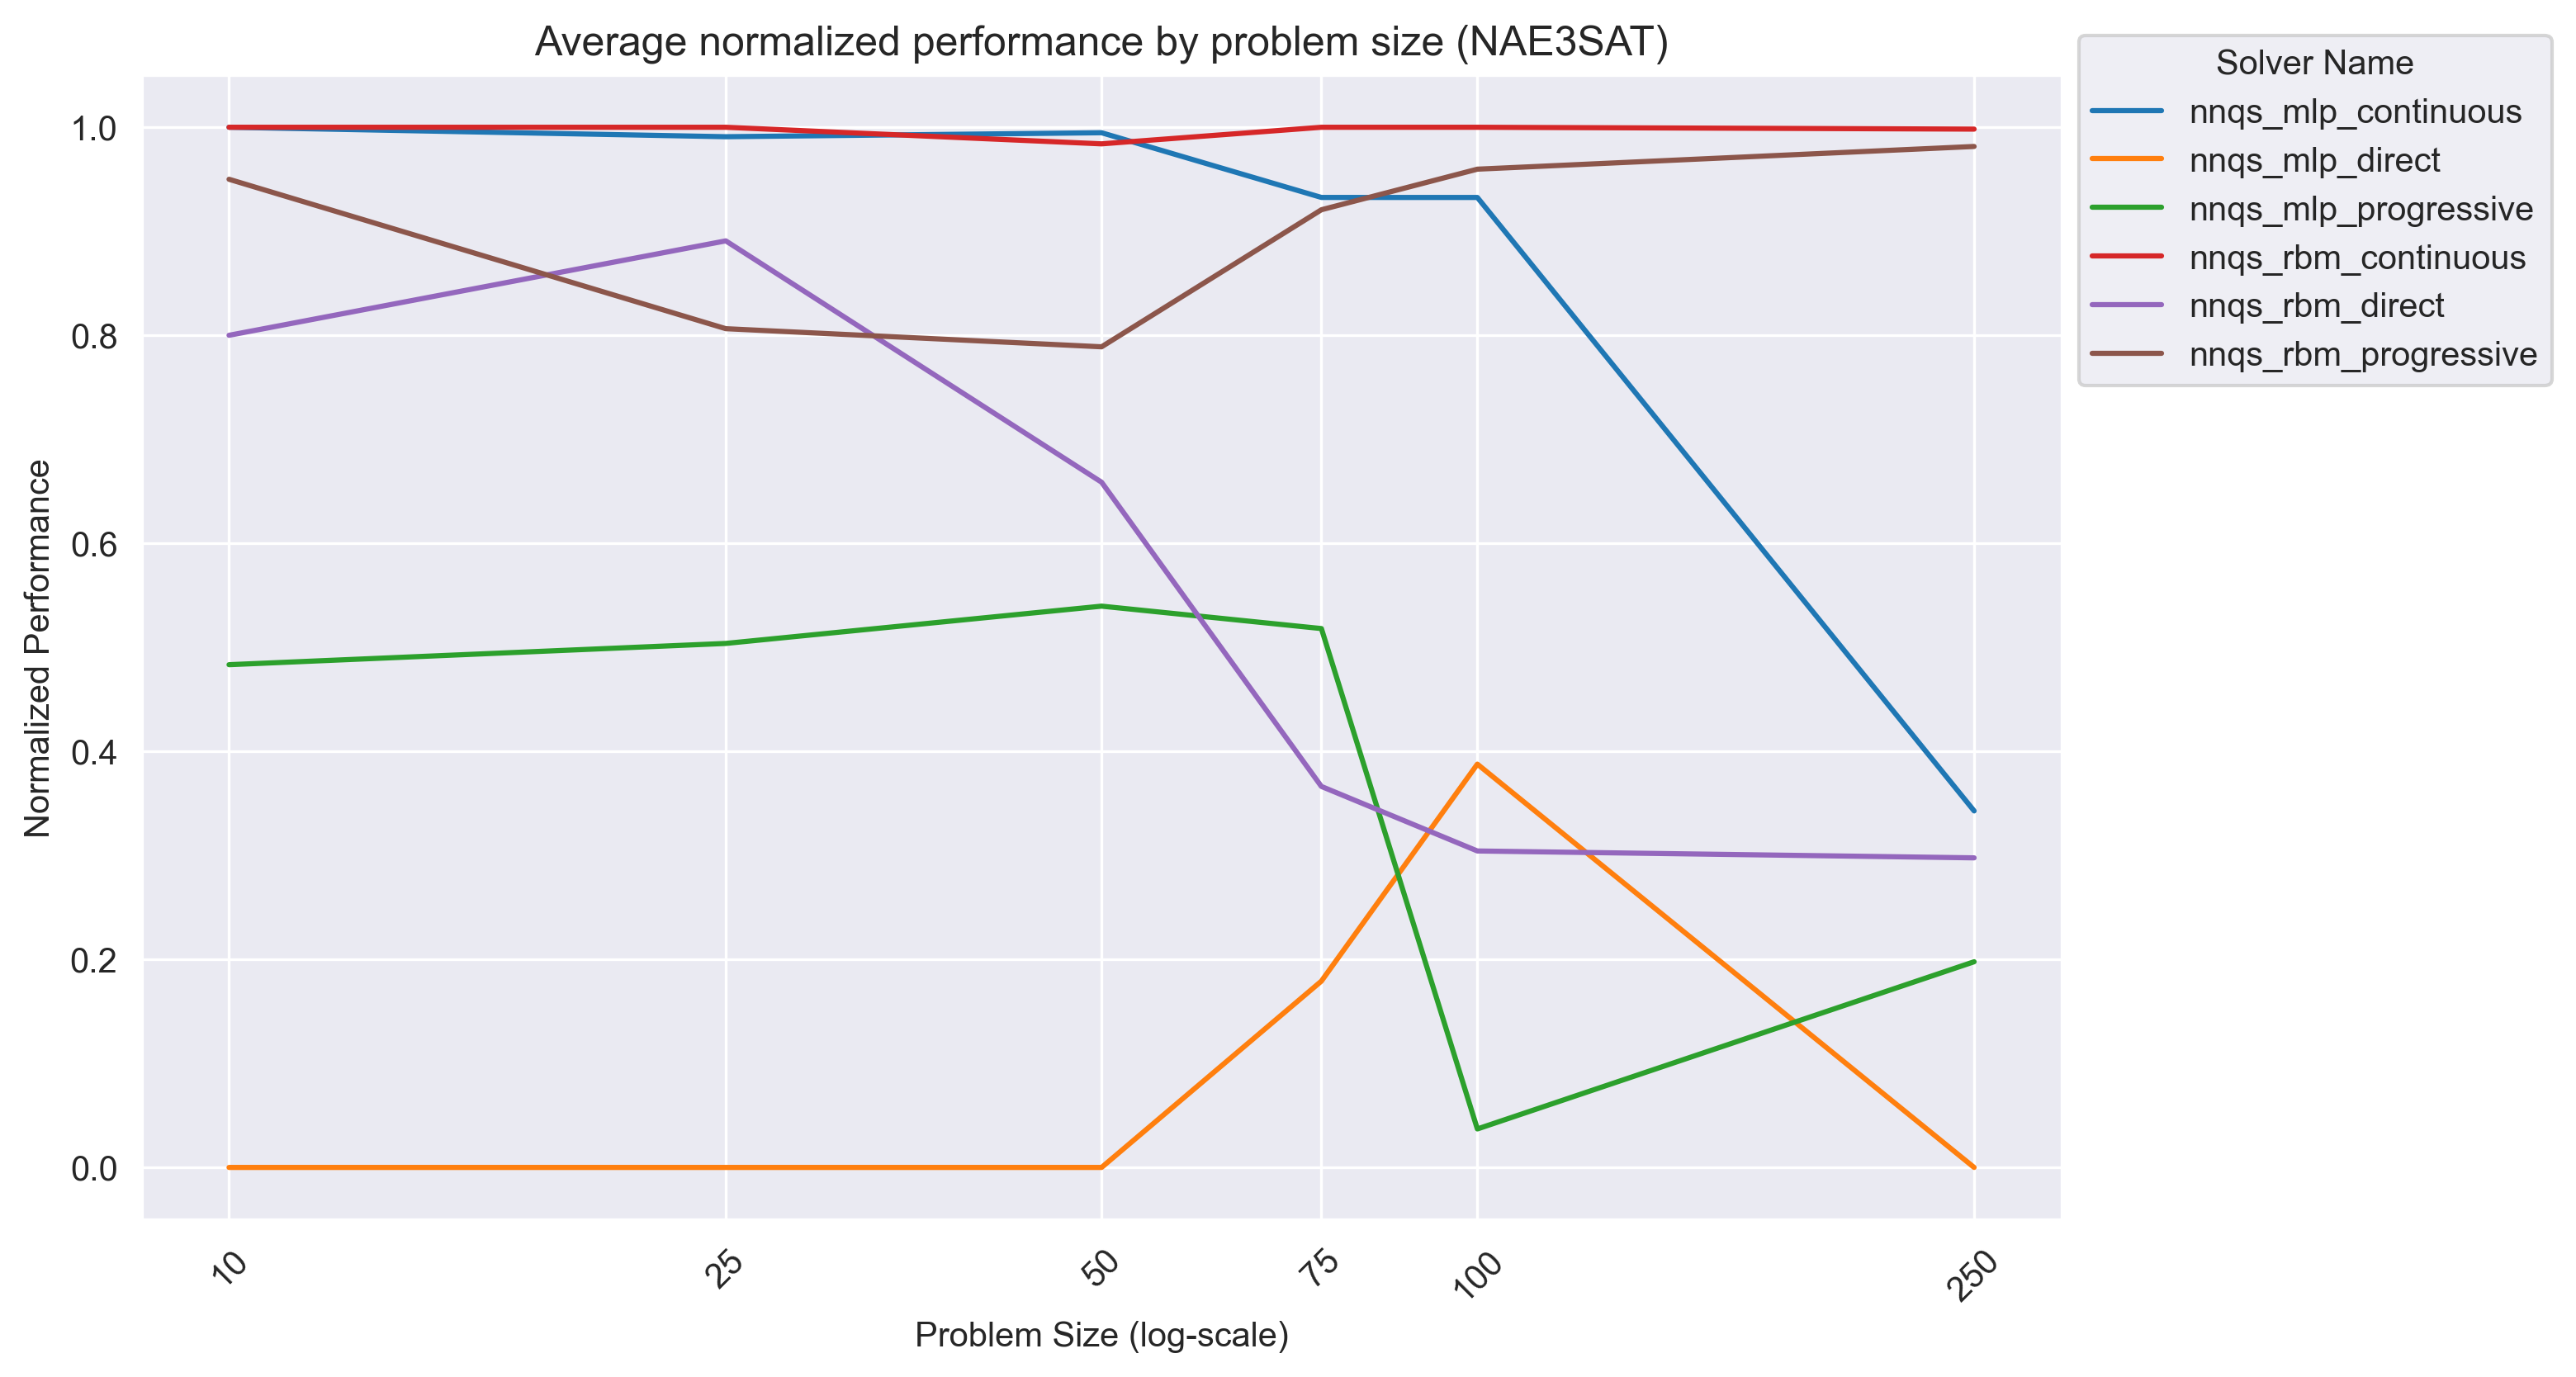
\includegraphics[width=0.9\textwidth]{images/nae3sat_nnqs_size.png}}
    \\
    \subfloat[Success probability]{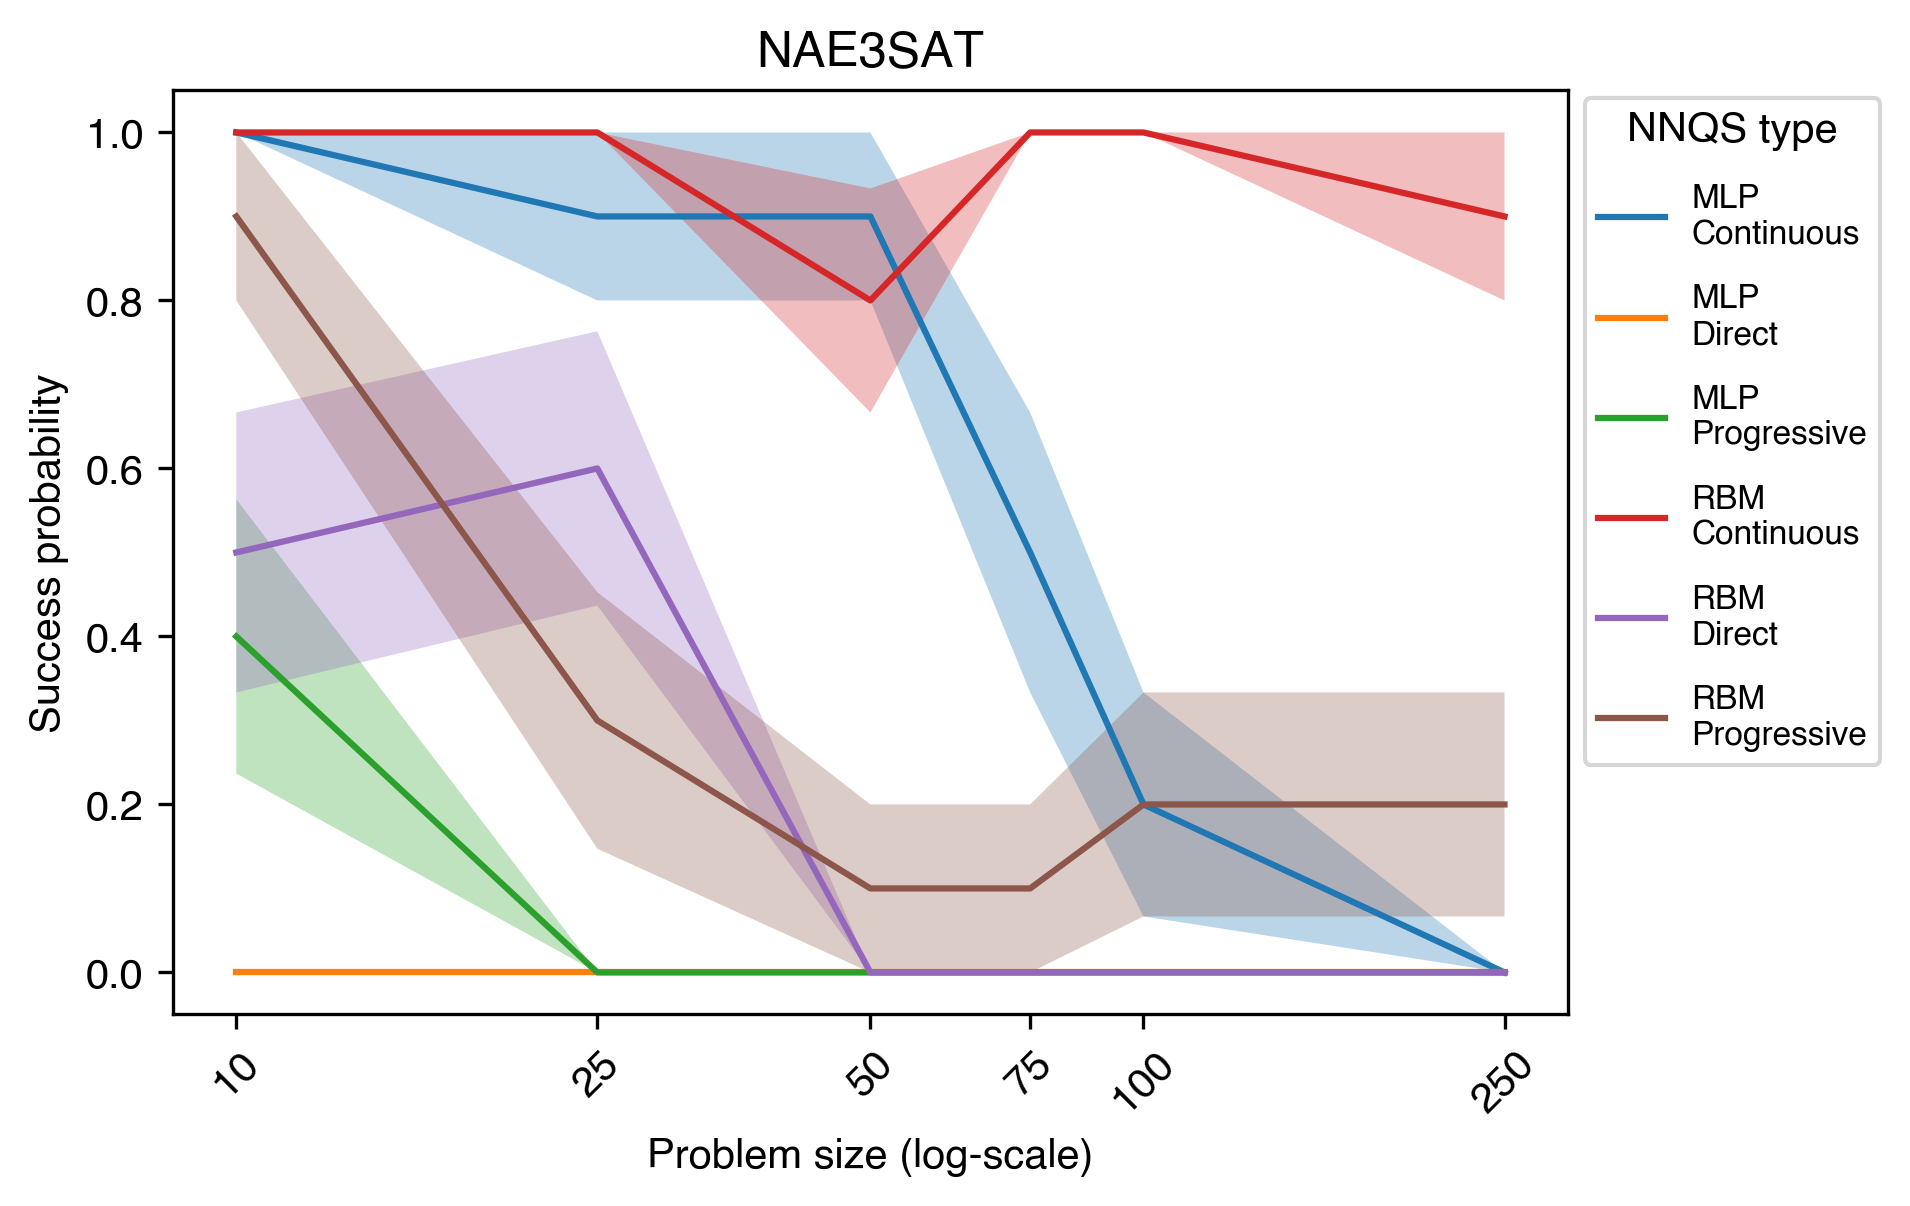
\includegraphics[width=0.9\textwidth]{images/nae3sat_nnqs_success_size.png}}
    \caption{Performance of different NNQS types for NAE3SAT by problem size}
    \label{nnqs-nae3sat-size}
\end{figure}

\begin{figure}[!htbp]
    \subfloat[Normalized energy]{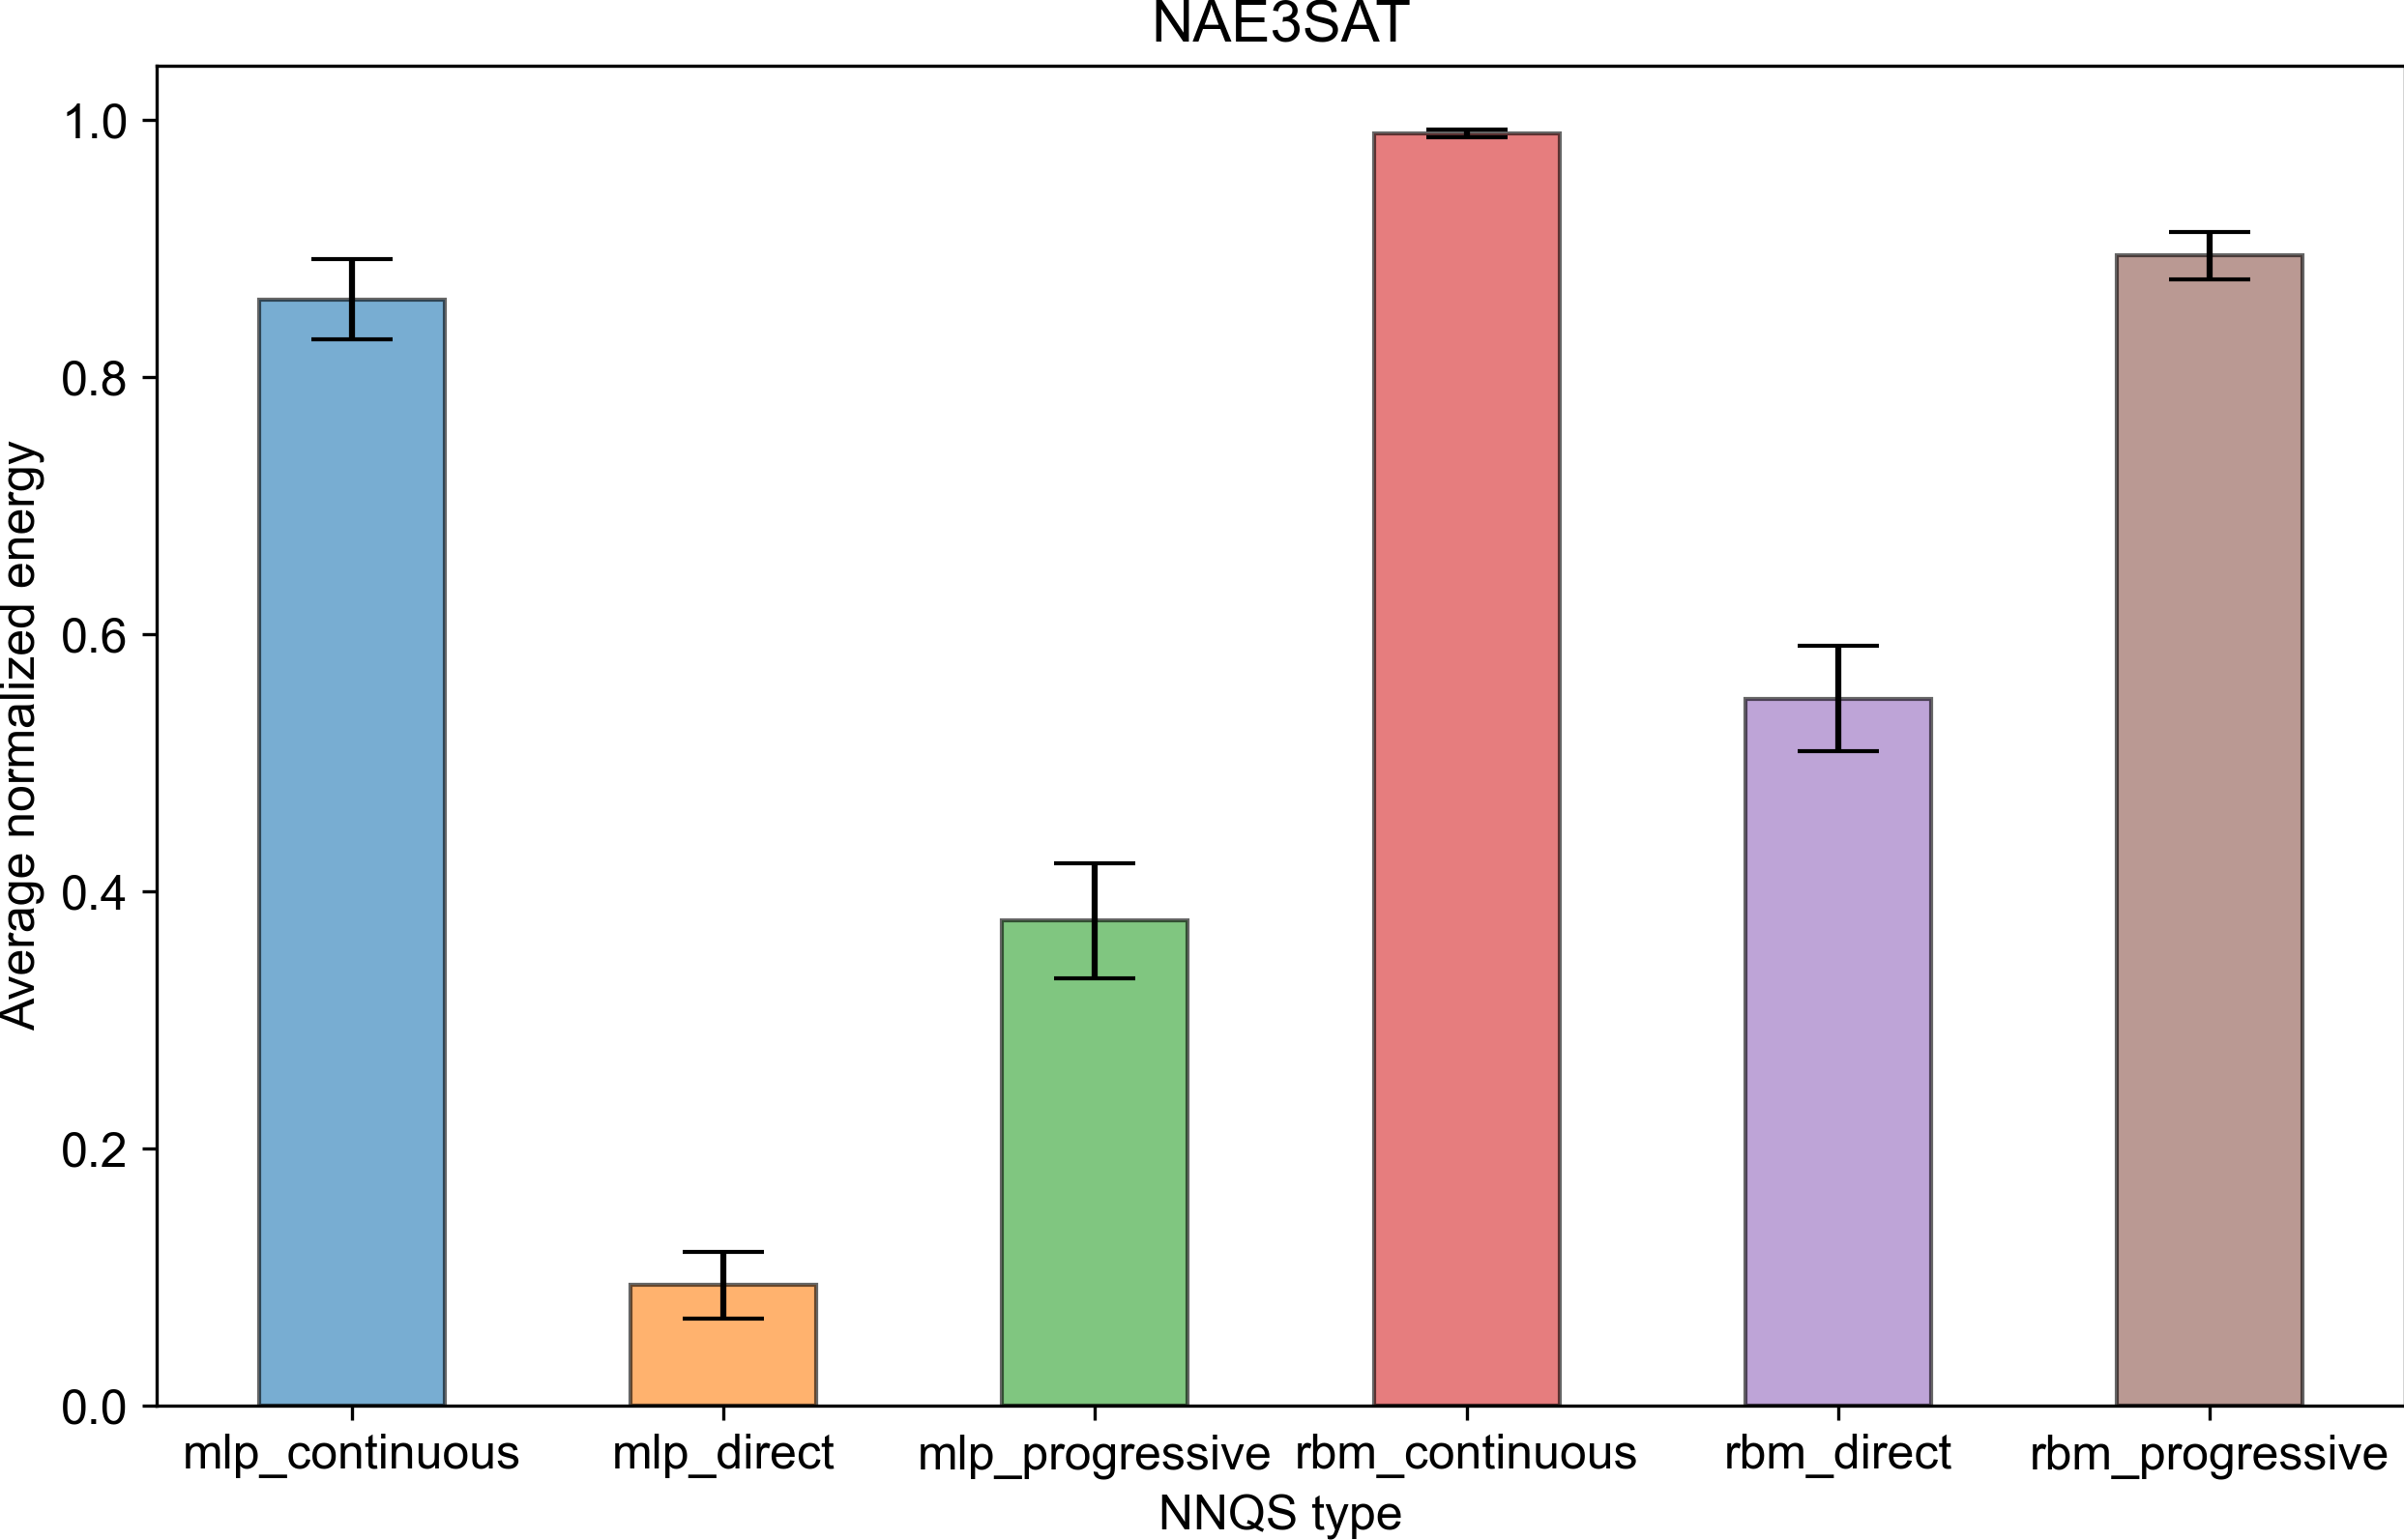
\includegraphics[width=0.49\textwidth]{images/nae3sat_nnqs_avg.png}}\hfill
    \subfloat[Success probability]{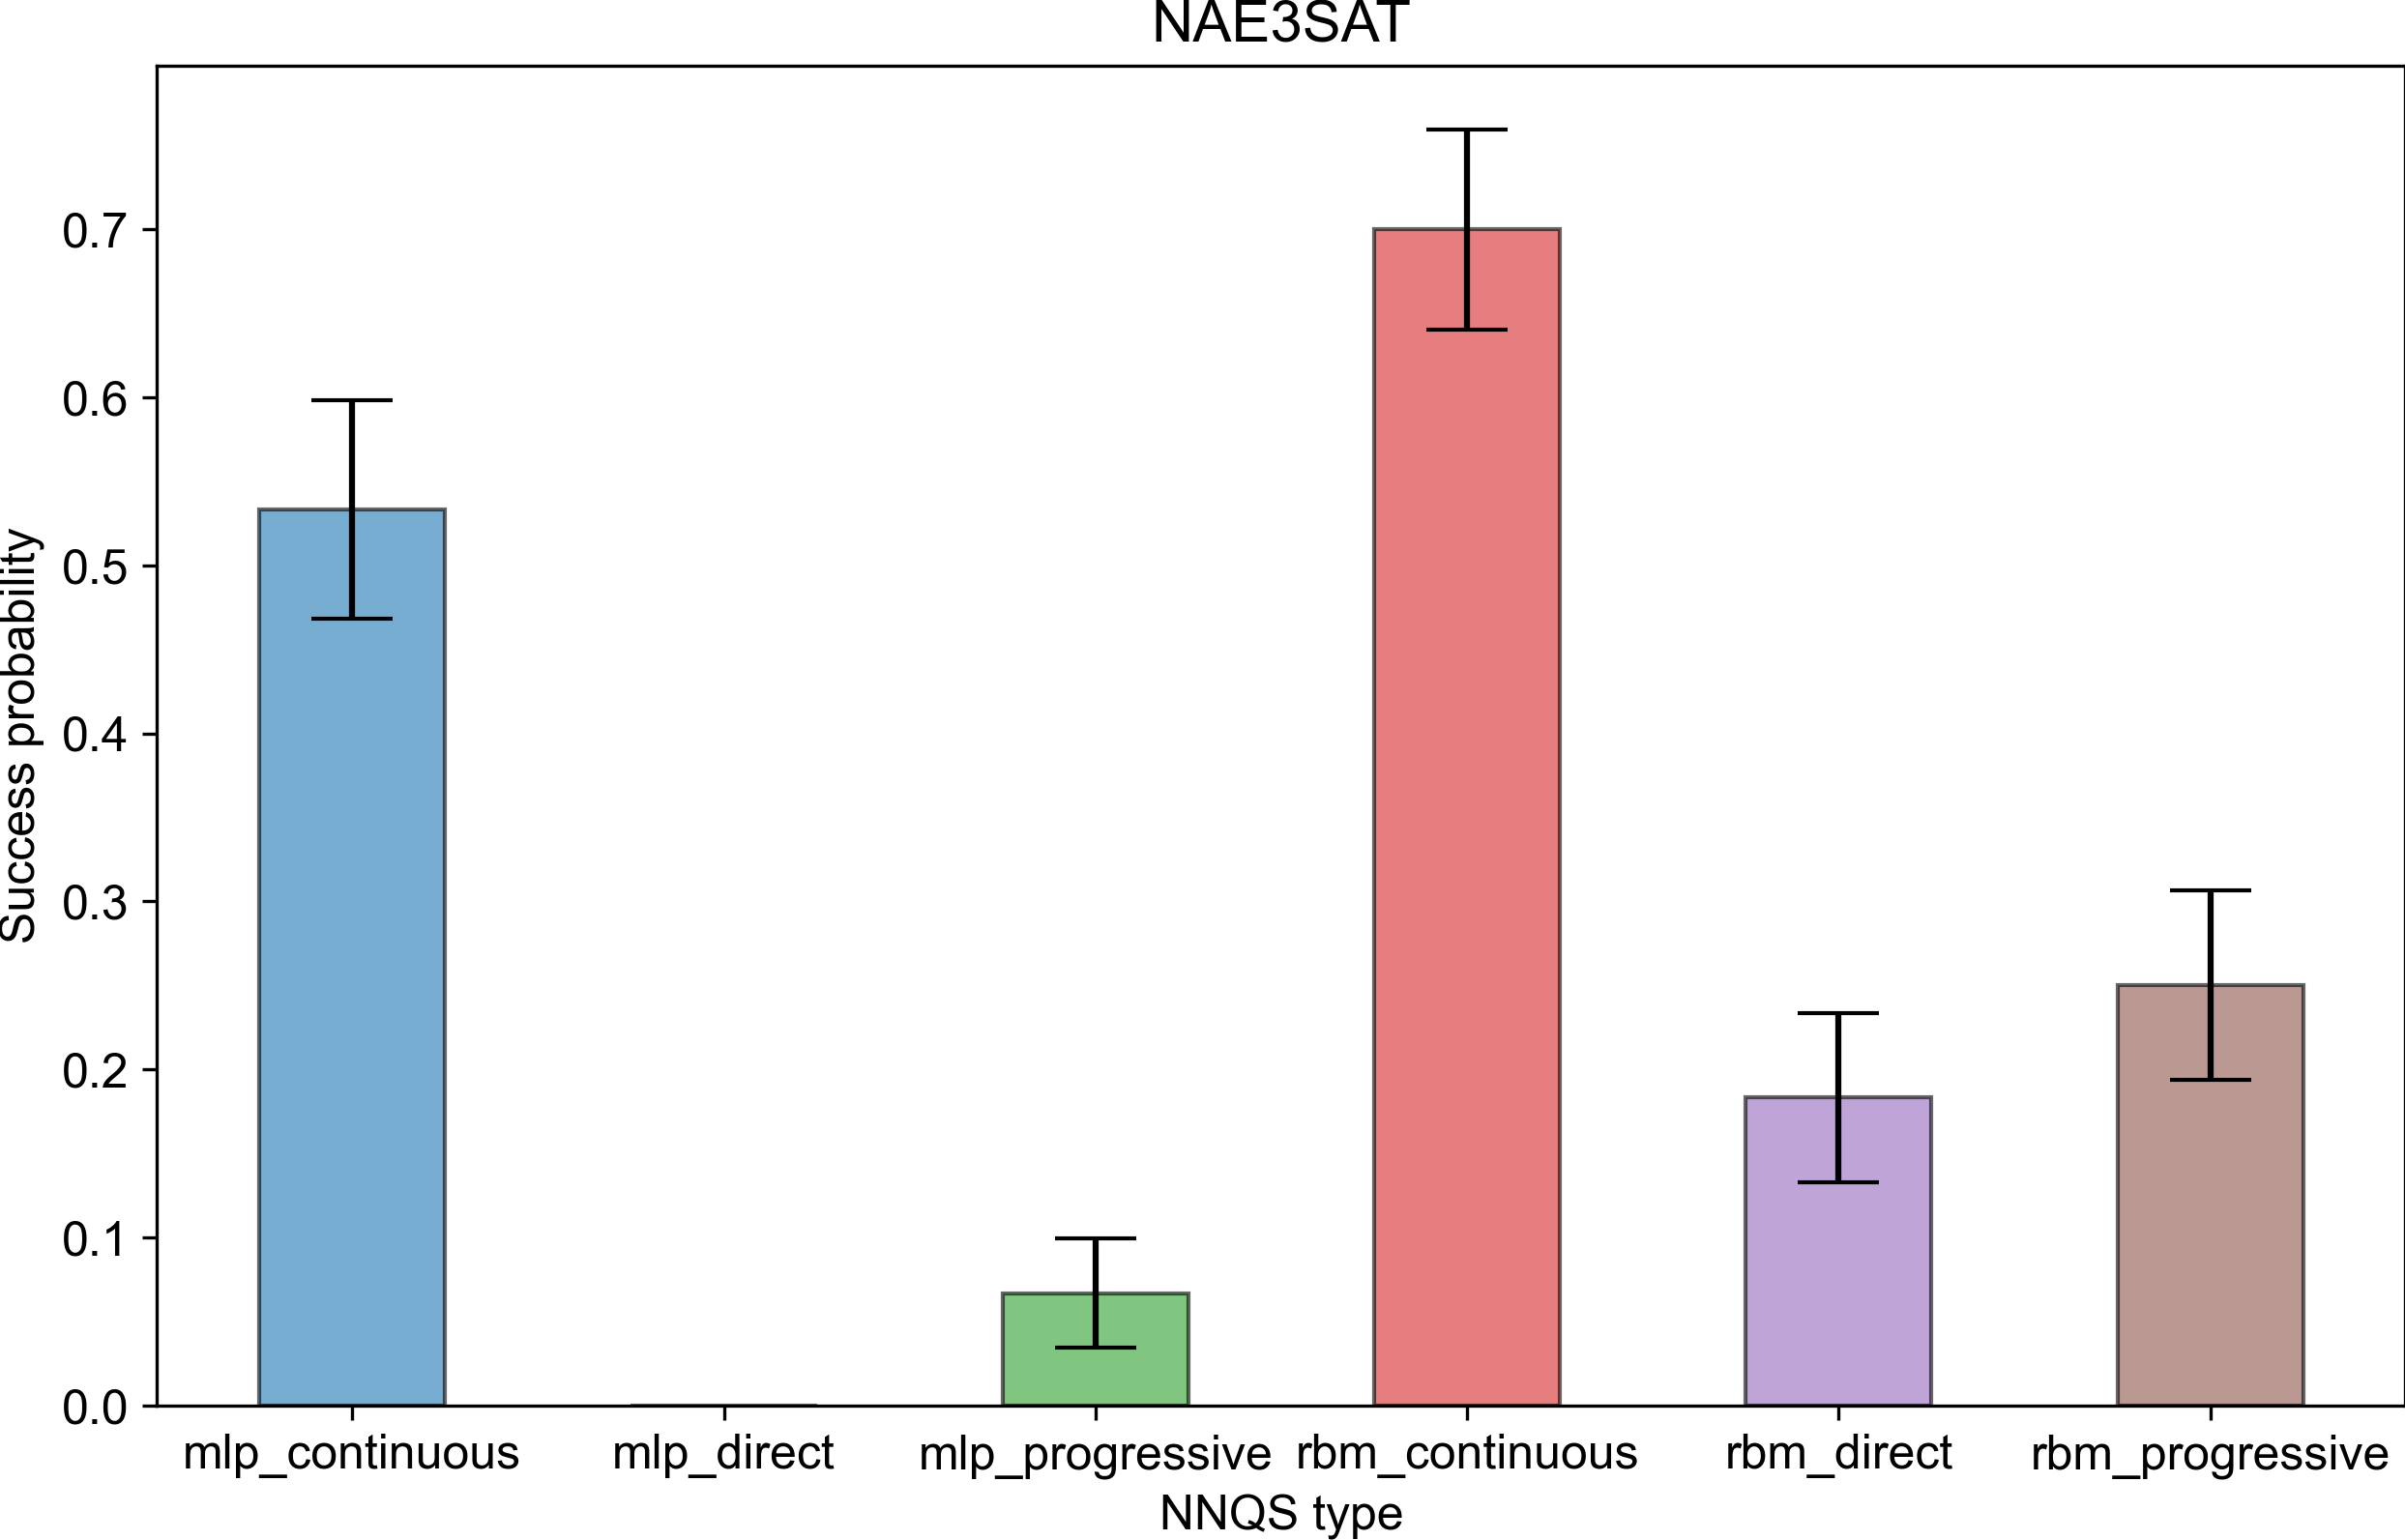
\includegraphics[width=0.49\textwidth]{images/nae3sat_nnqs_success_avg.png}}
    \caption{Average performance of different NNQS types for NAE3SAT}
    \label{nnqs-nae3sat-average}
\end{figure}

For the NAE3SAT dataset, the continuous training algorithm with the RBM performed the best in terms of normalized energy and success probability, shown in \autoref{nnqs-nae3sat-size}, except with a problem size of $50$. This is likely due to variance in the randomly generated data set. The performance averaged across all sizes, shown in \autoref{nnqs-nae3sat-average}, also highlights that the RBM with a continuous training algorithm performs the best.

\subsection{Max-cut}

\begin{figure}[!htbp]
    \subfloat[Normalized energy]{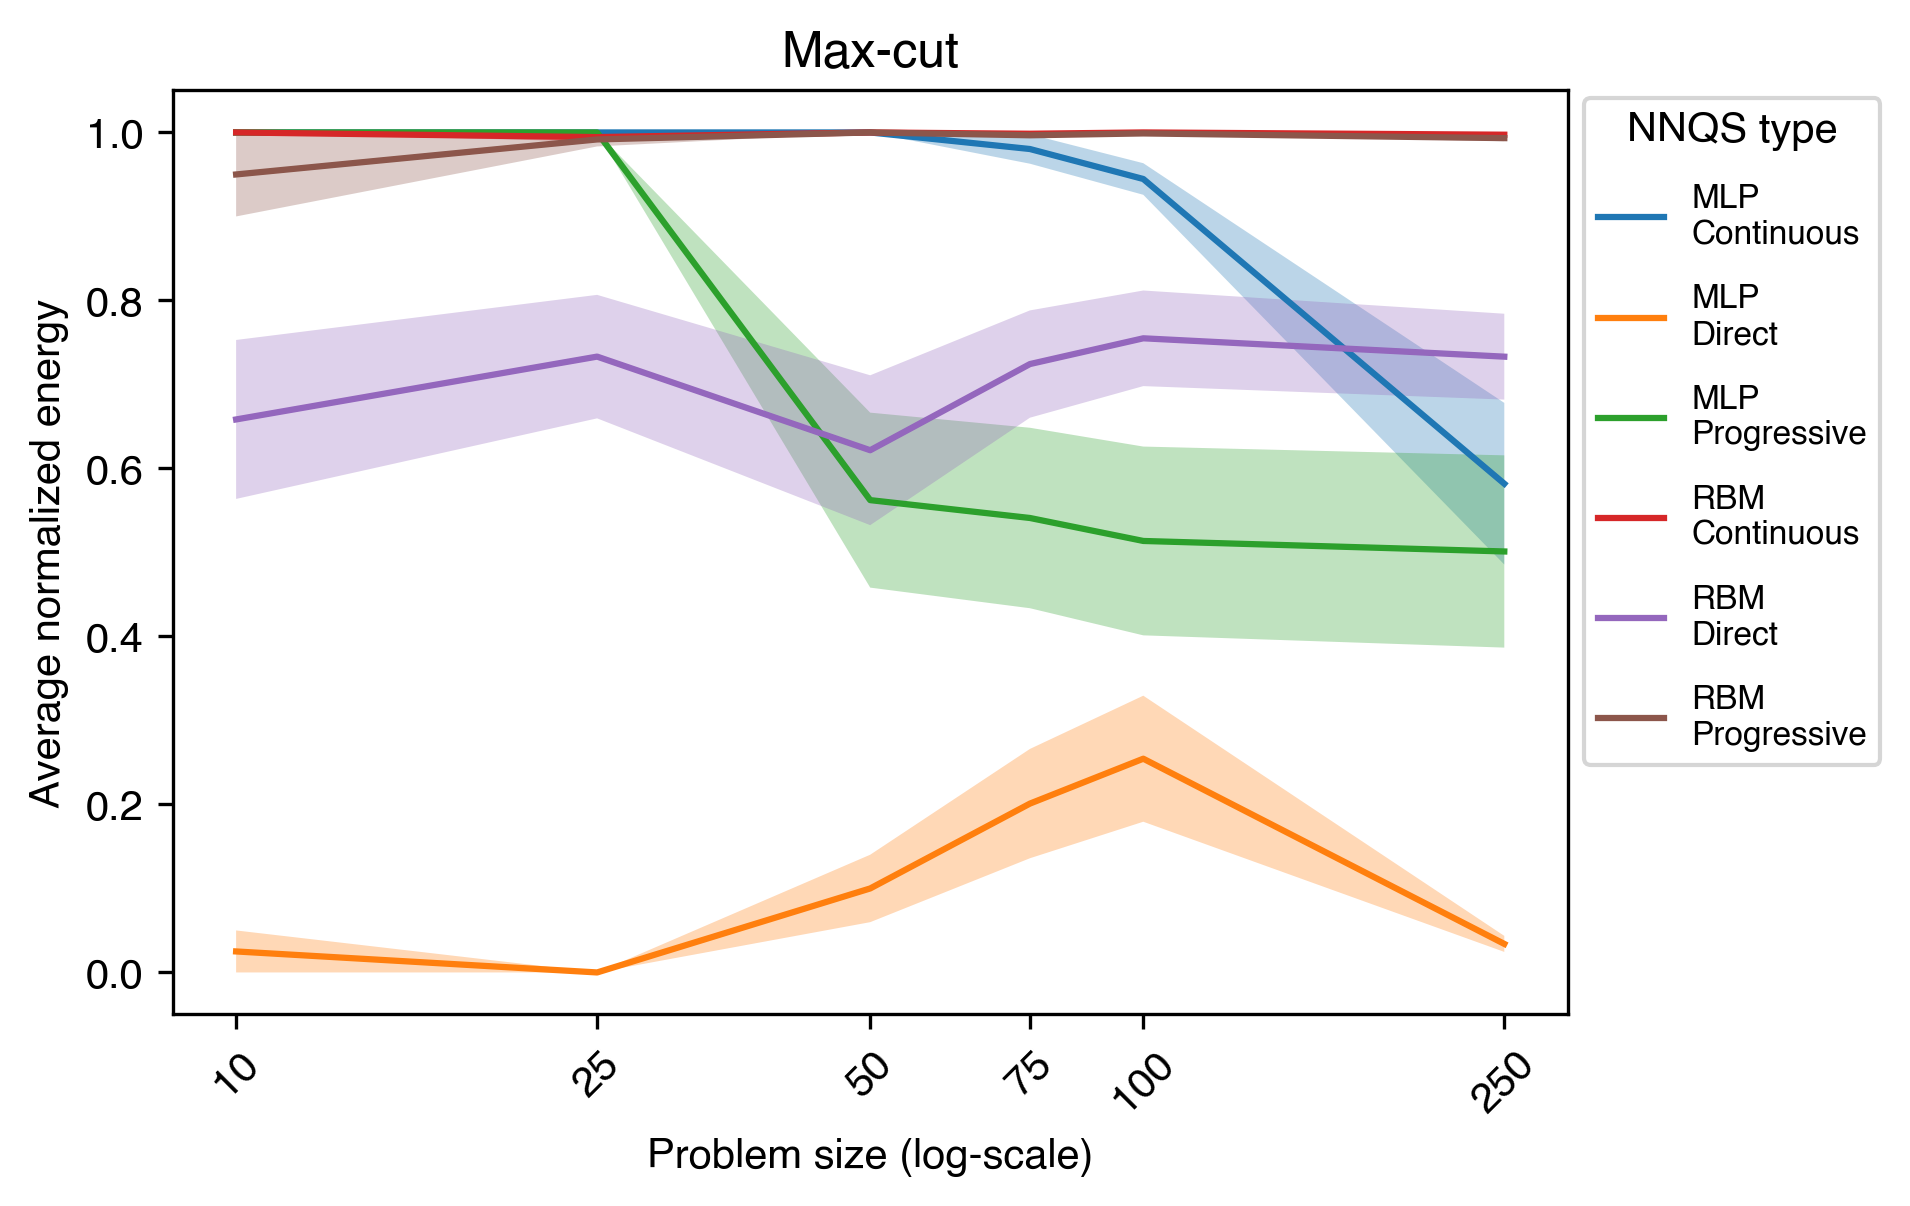
\includegraphics[width=0.9\textwidth]{images/maxcut_nnqs_size.png}}
    \\
    \subfloat[Success probability]{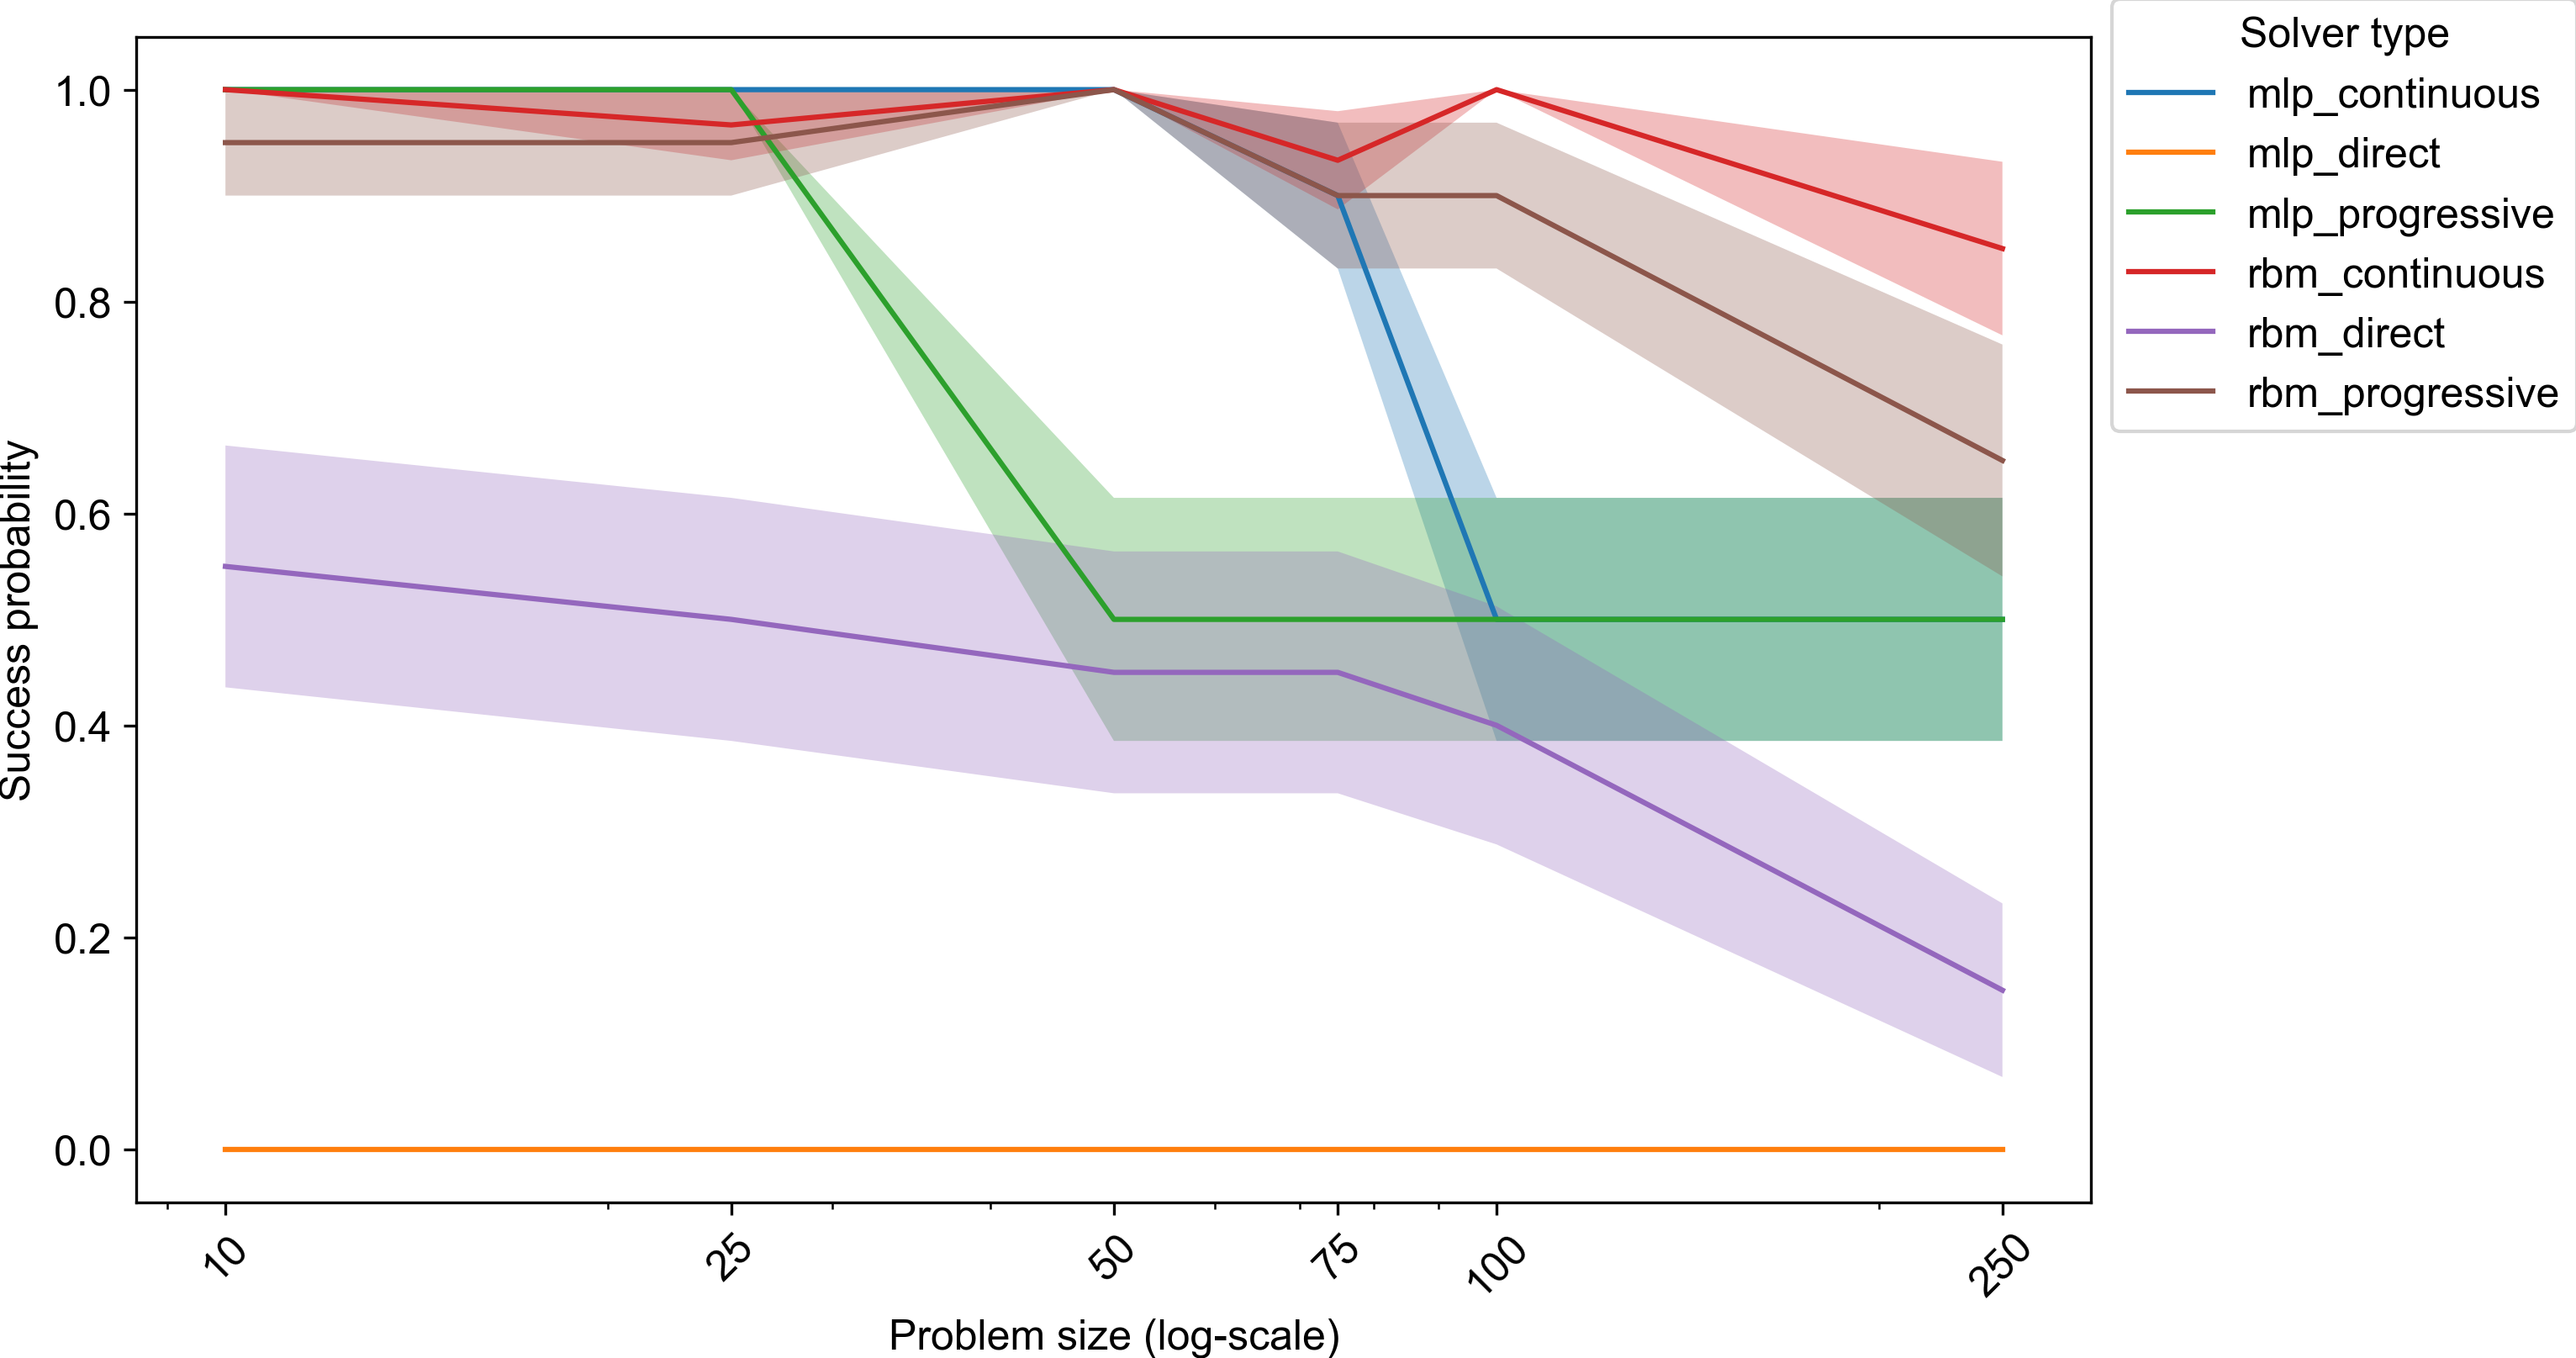
\includegraphics[width=0.9\textwidth]{images/maxcut_nnqs_success_size.png}}
    \caption{Performance of different NNQS types for max-cut by problem size}
    \label{nnqs-maxcut-size}
\end{figure}

\begin{figure}[!htbp]
    \subfloat[Normalized energy]{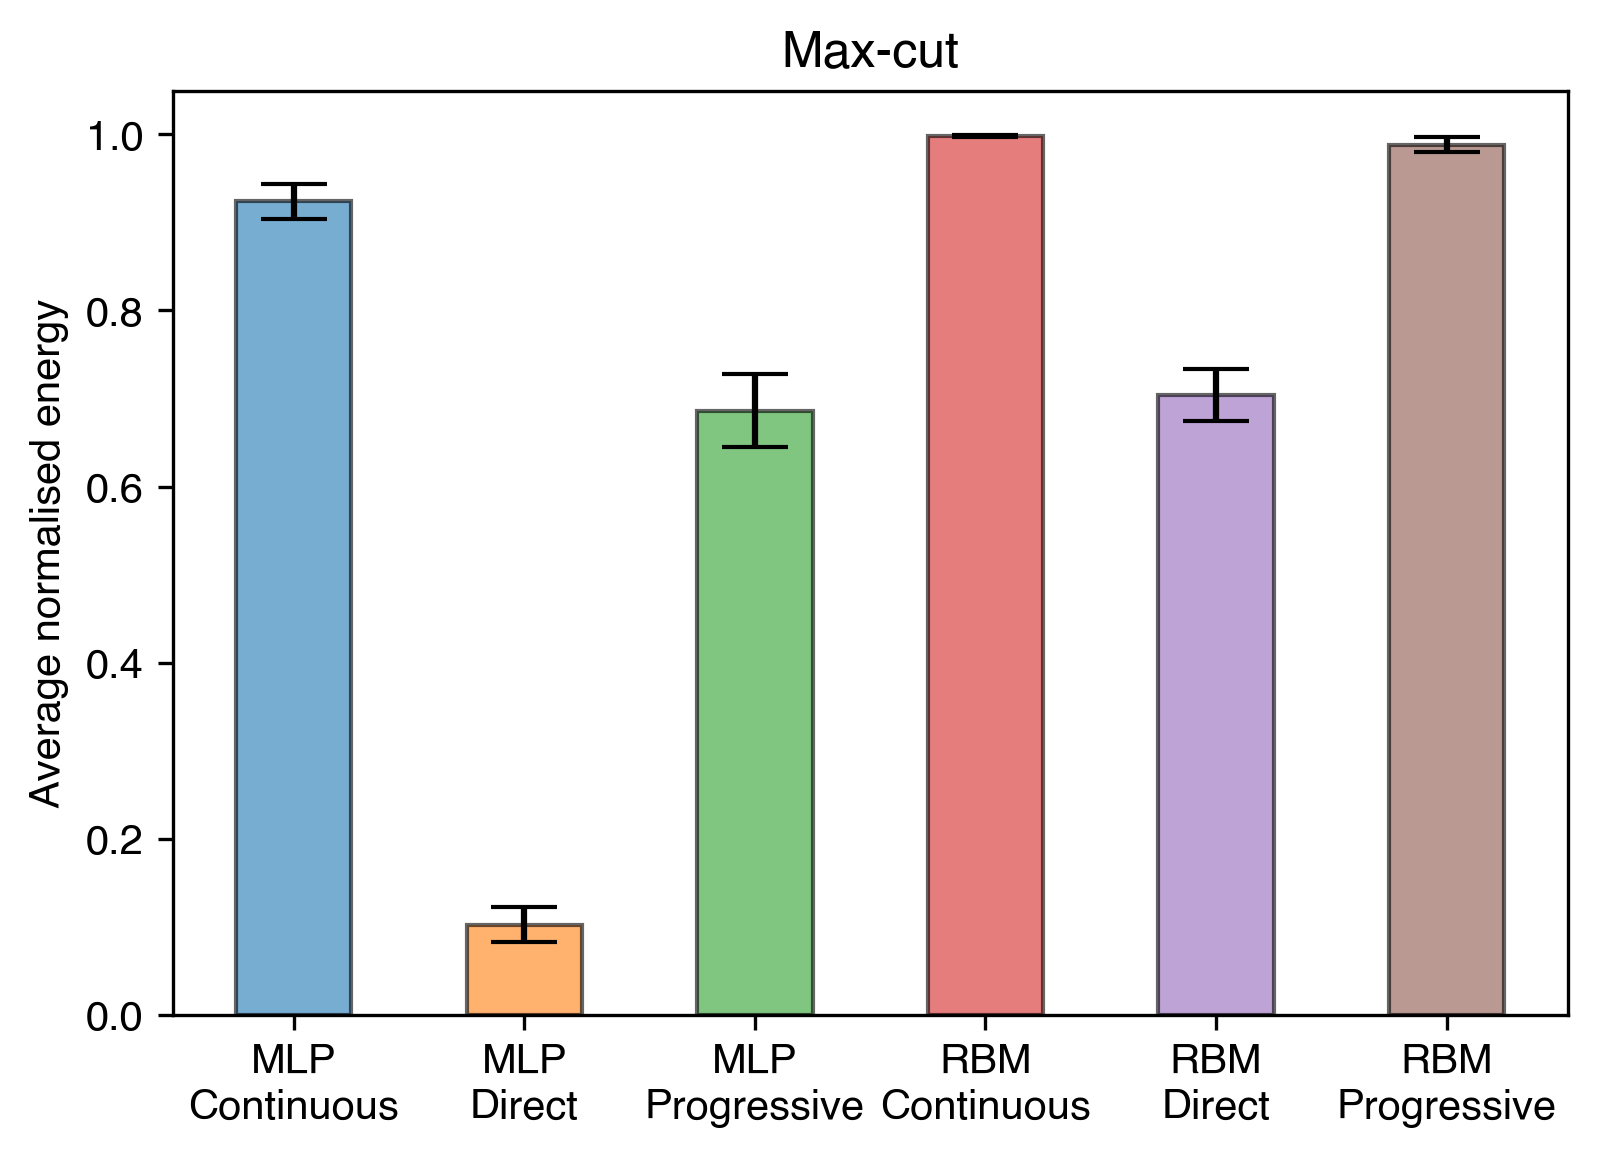
\includegraphics[width=0.49\textwidth]{images/maxcut_nnqs_avg.png}}\hfill
    \subfloat[Success probability]{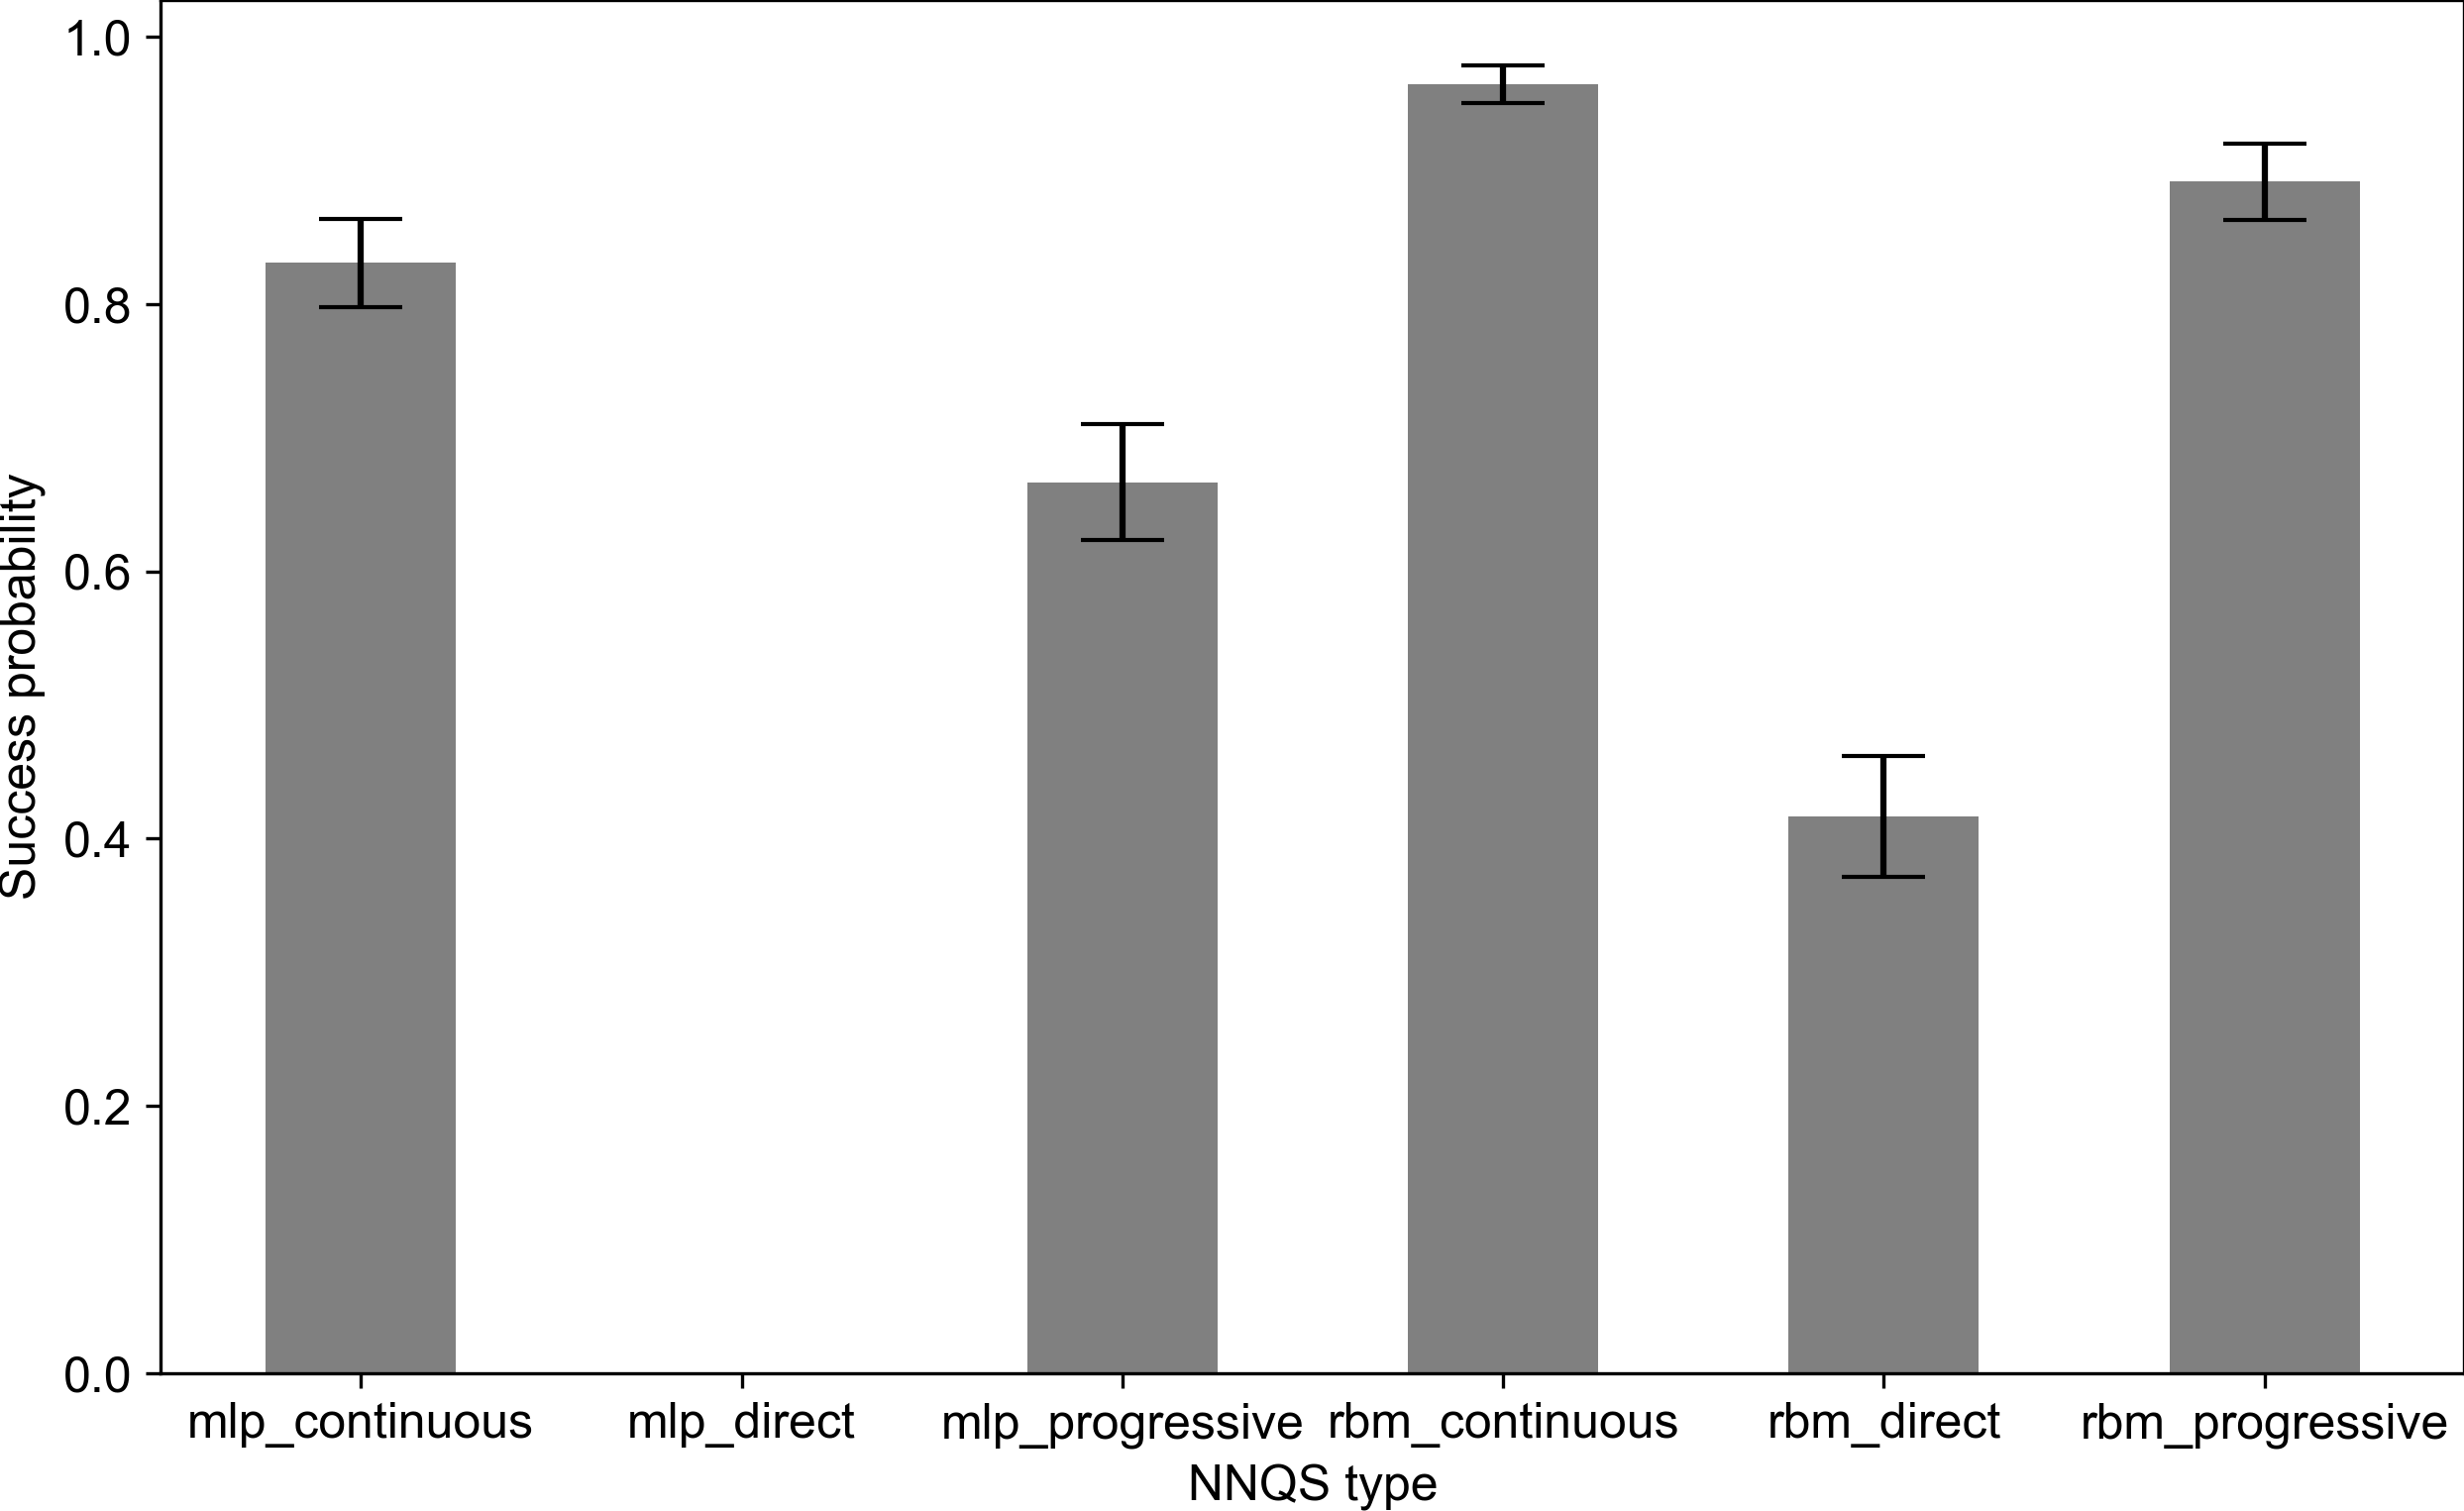
\includegraphics[width=0.49\textwidth]{images/maxcut_nnqs_success_avg.png}}
    \caption{Average performance of different NNQS types for max-cut}
    \label{nnqs-maxcut-average}
\end{figure}

For the max-cut dataset, the continuous training algorithm with the RBM generally performed the best in terms of normalized energy and success probability, shown in \autoref{nnqs-maxcut-size}, except with a problem size of $25$. This is likely due to variance in the randomly generated data set. The performance averaged across all sizes, shown in \autoref{nnqs-maxcut-average}, also highlights that the RBM with a continuous training algorithm performs the best. However, the gap in success probability between the models is relatively small and this likely implies that the max-cut problem is easier in general compared to the NAE3SAT problem.


\subsection{SK model}

\begin{figure}[!htbp]
    \centering
    \subfloat[Normalized energy]{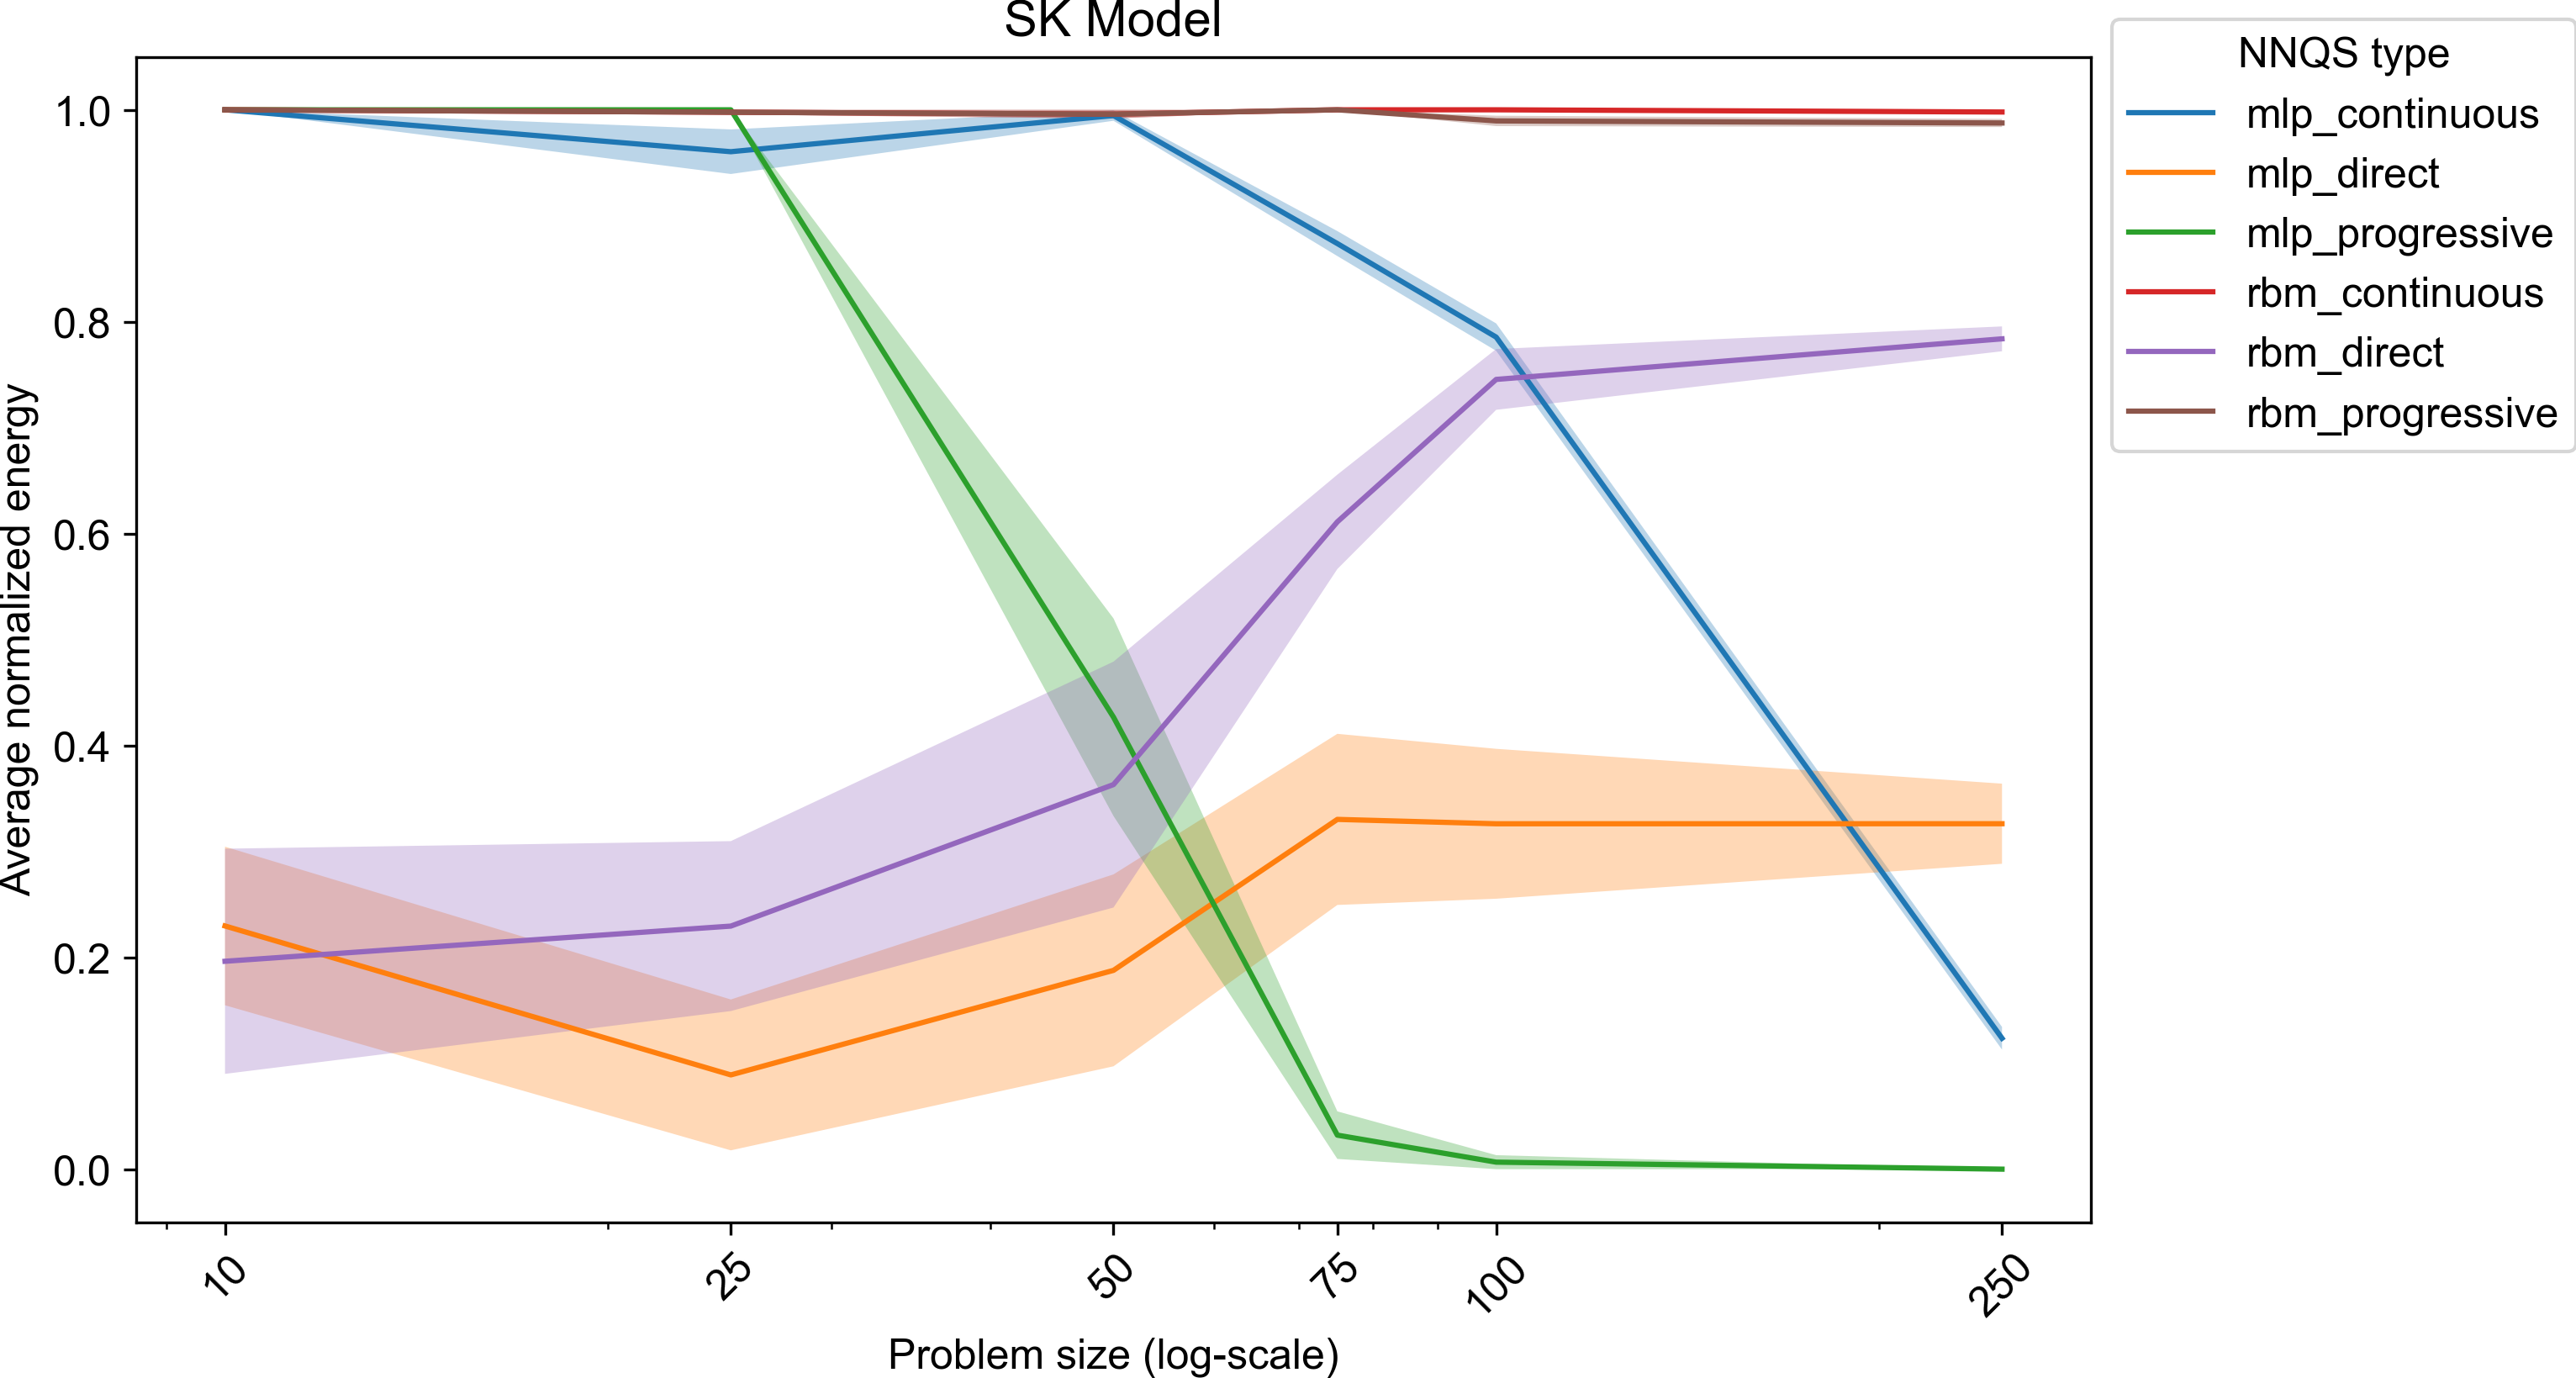
\includegraphics[width=0.9\textwidth]{images/skmodel_nnqs_size.png}}%\hfill
    \\
    \subfloat[Success probability]{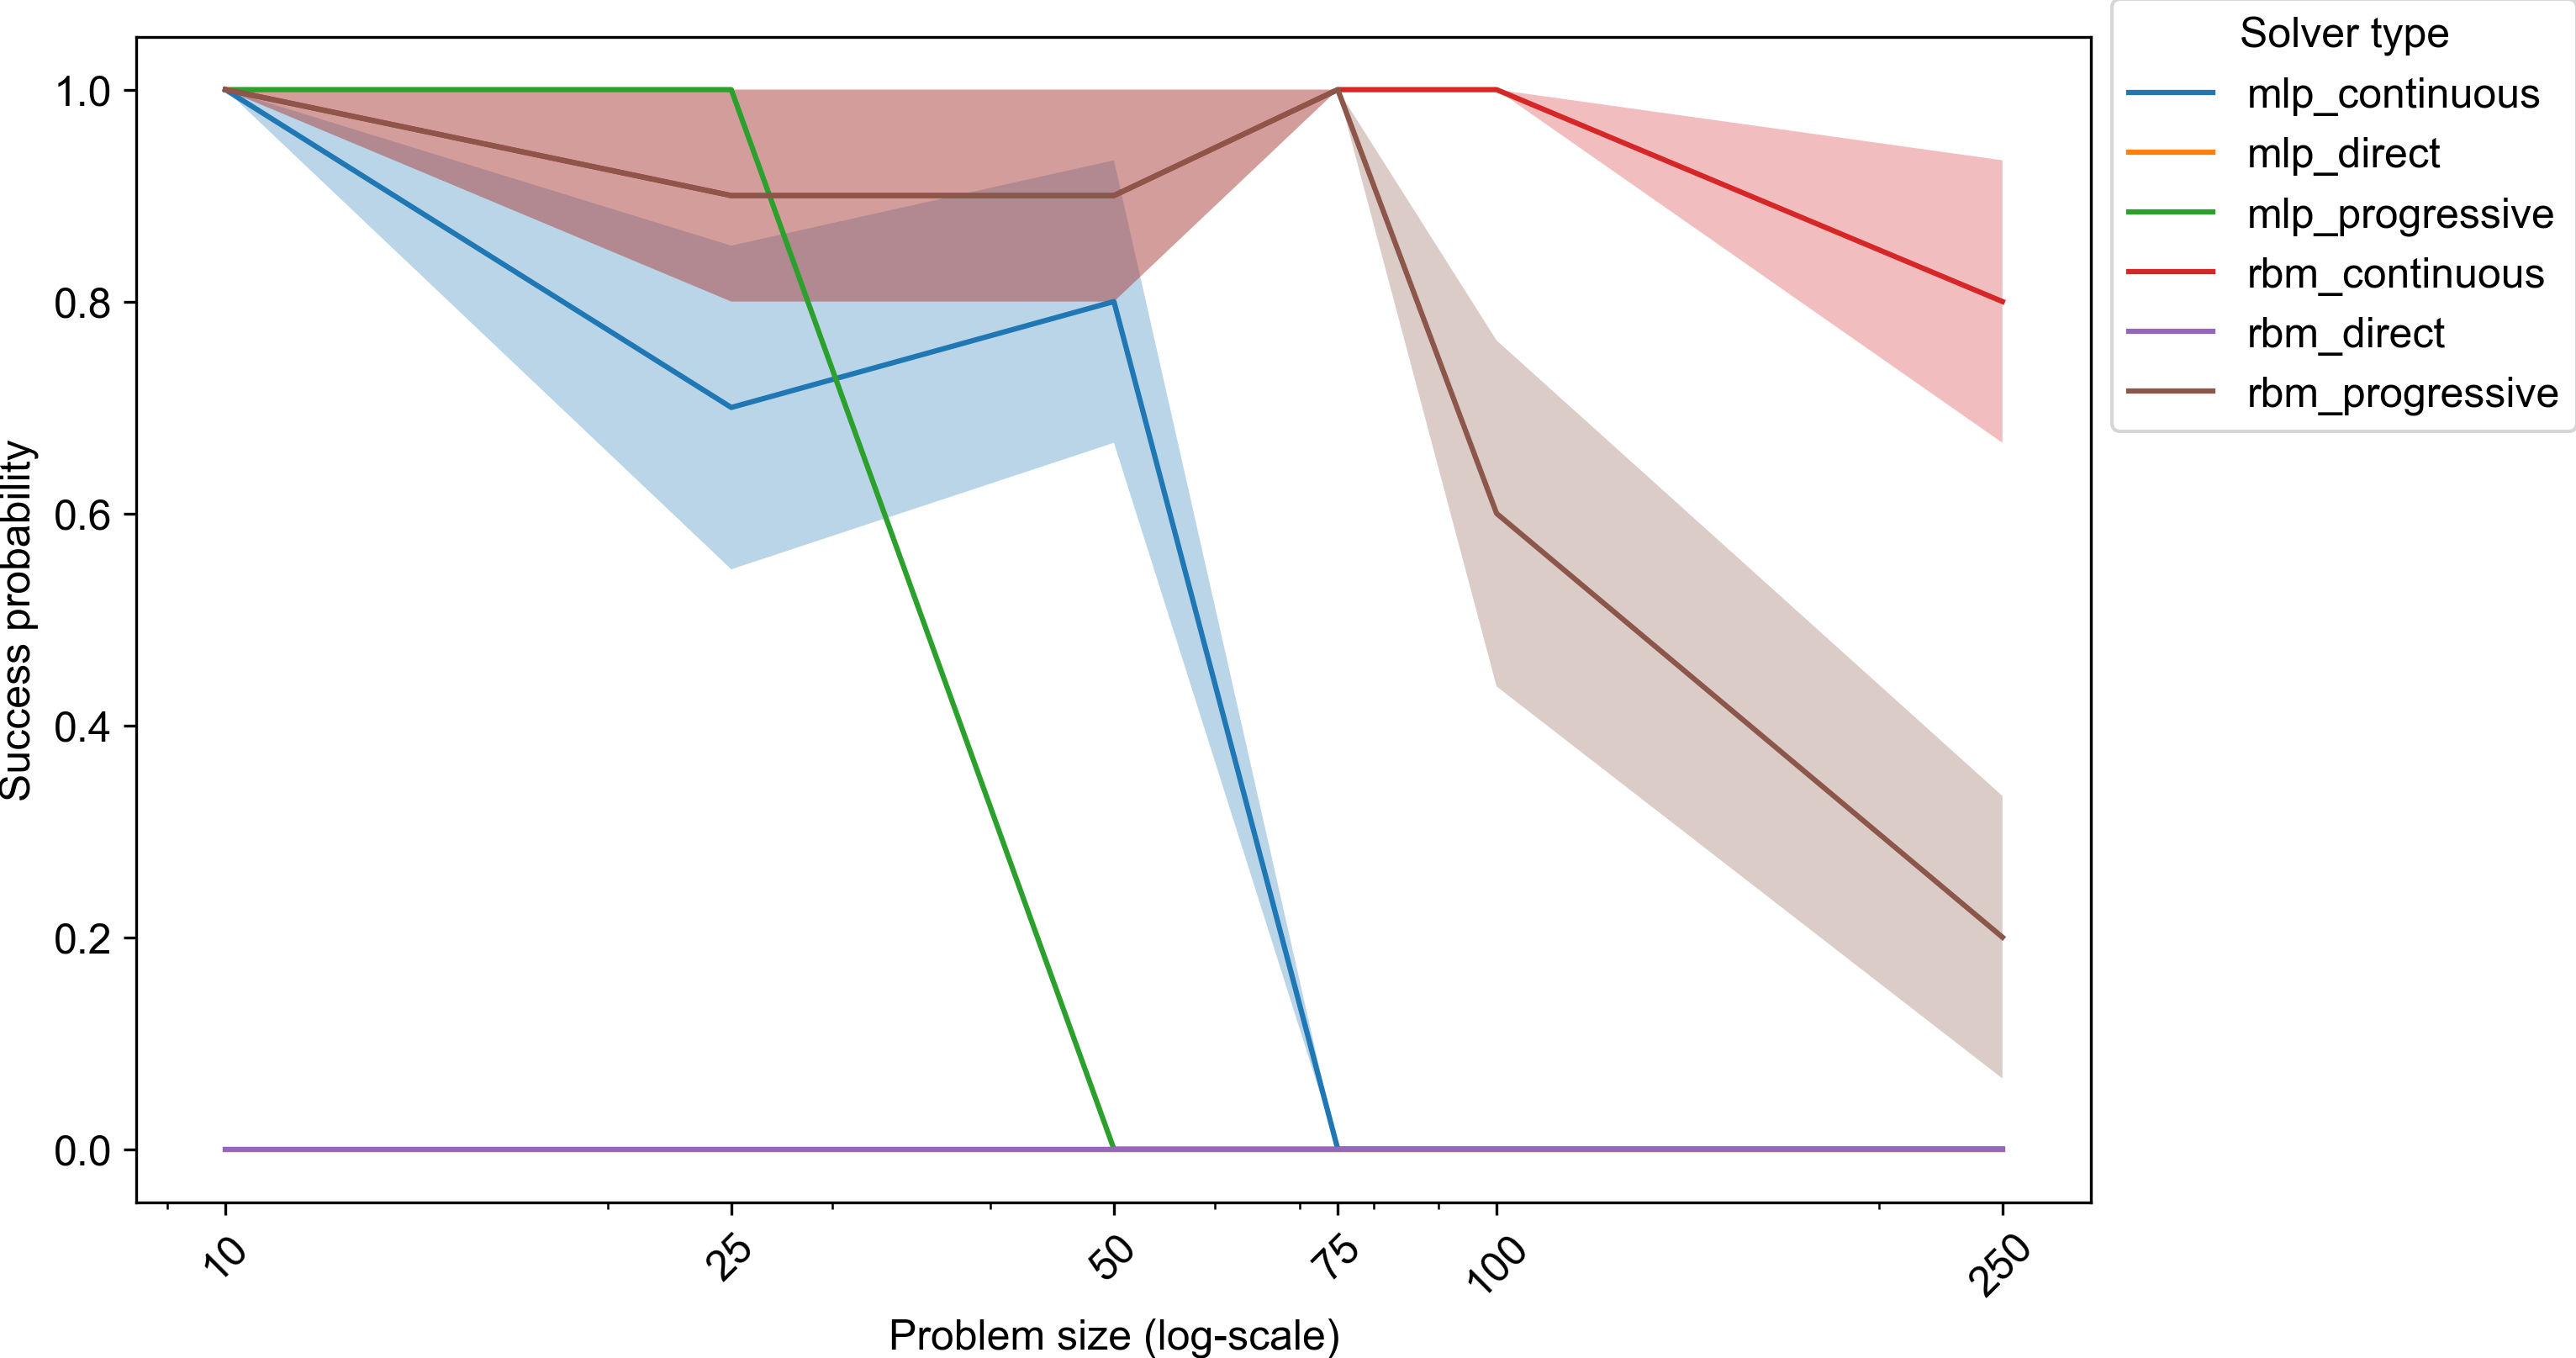
\includegraphics[width=0.9\textwidth]{images/skmodel_nnqs_success_size.png}}
    \caption{Performance of different NNQS types for SK model by problem size}
    \label{nnqs-skmodel-size}
\end{figure}

\begin{figure}[!htbp]
    \subfloat[Normalized energy]{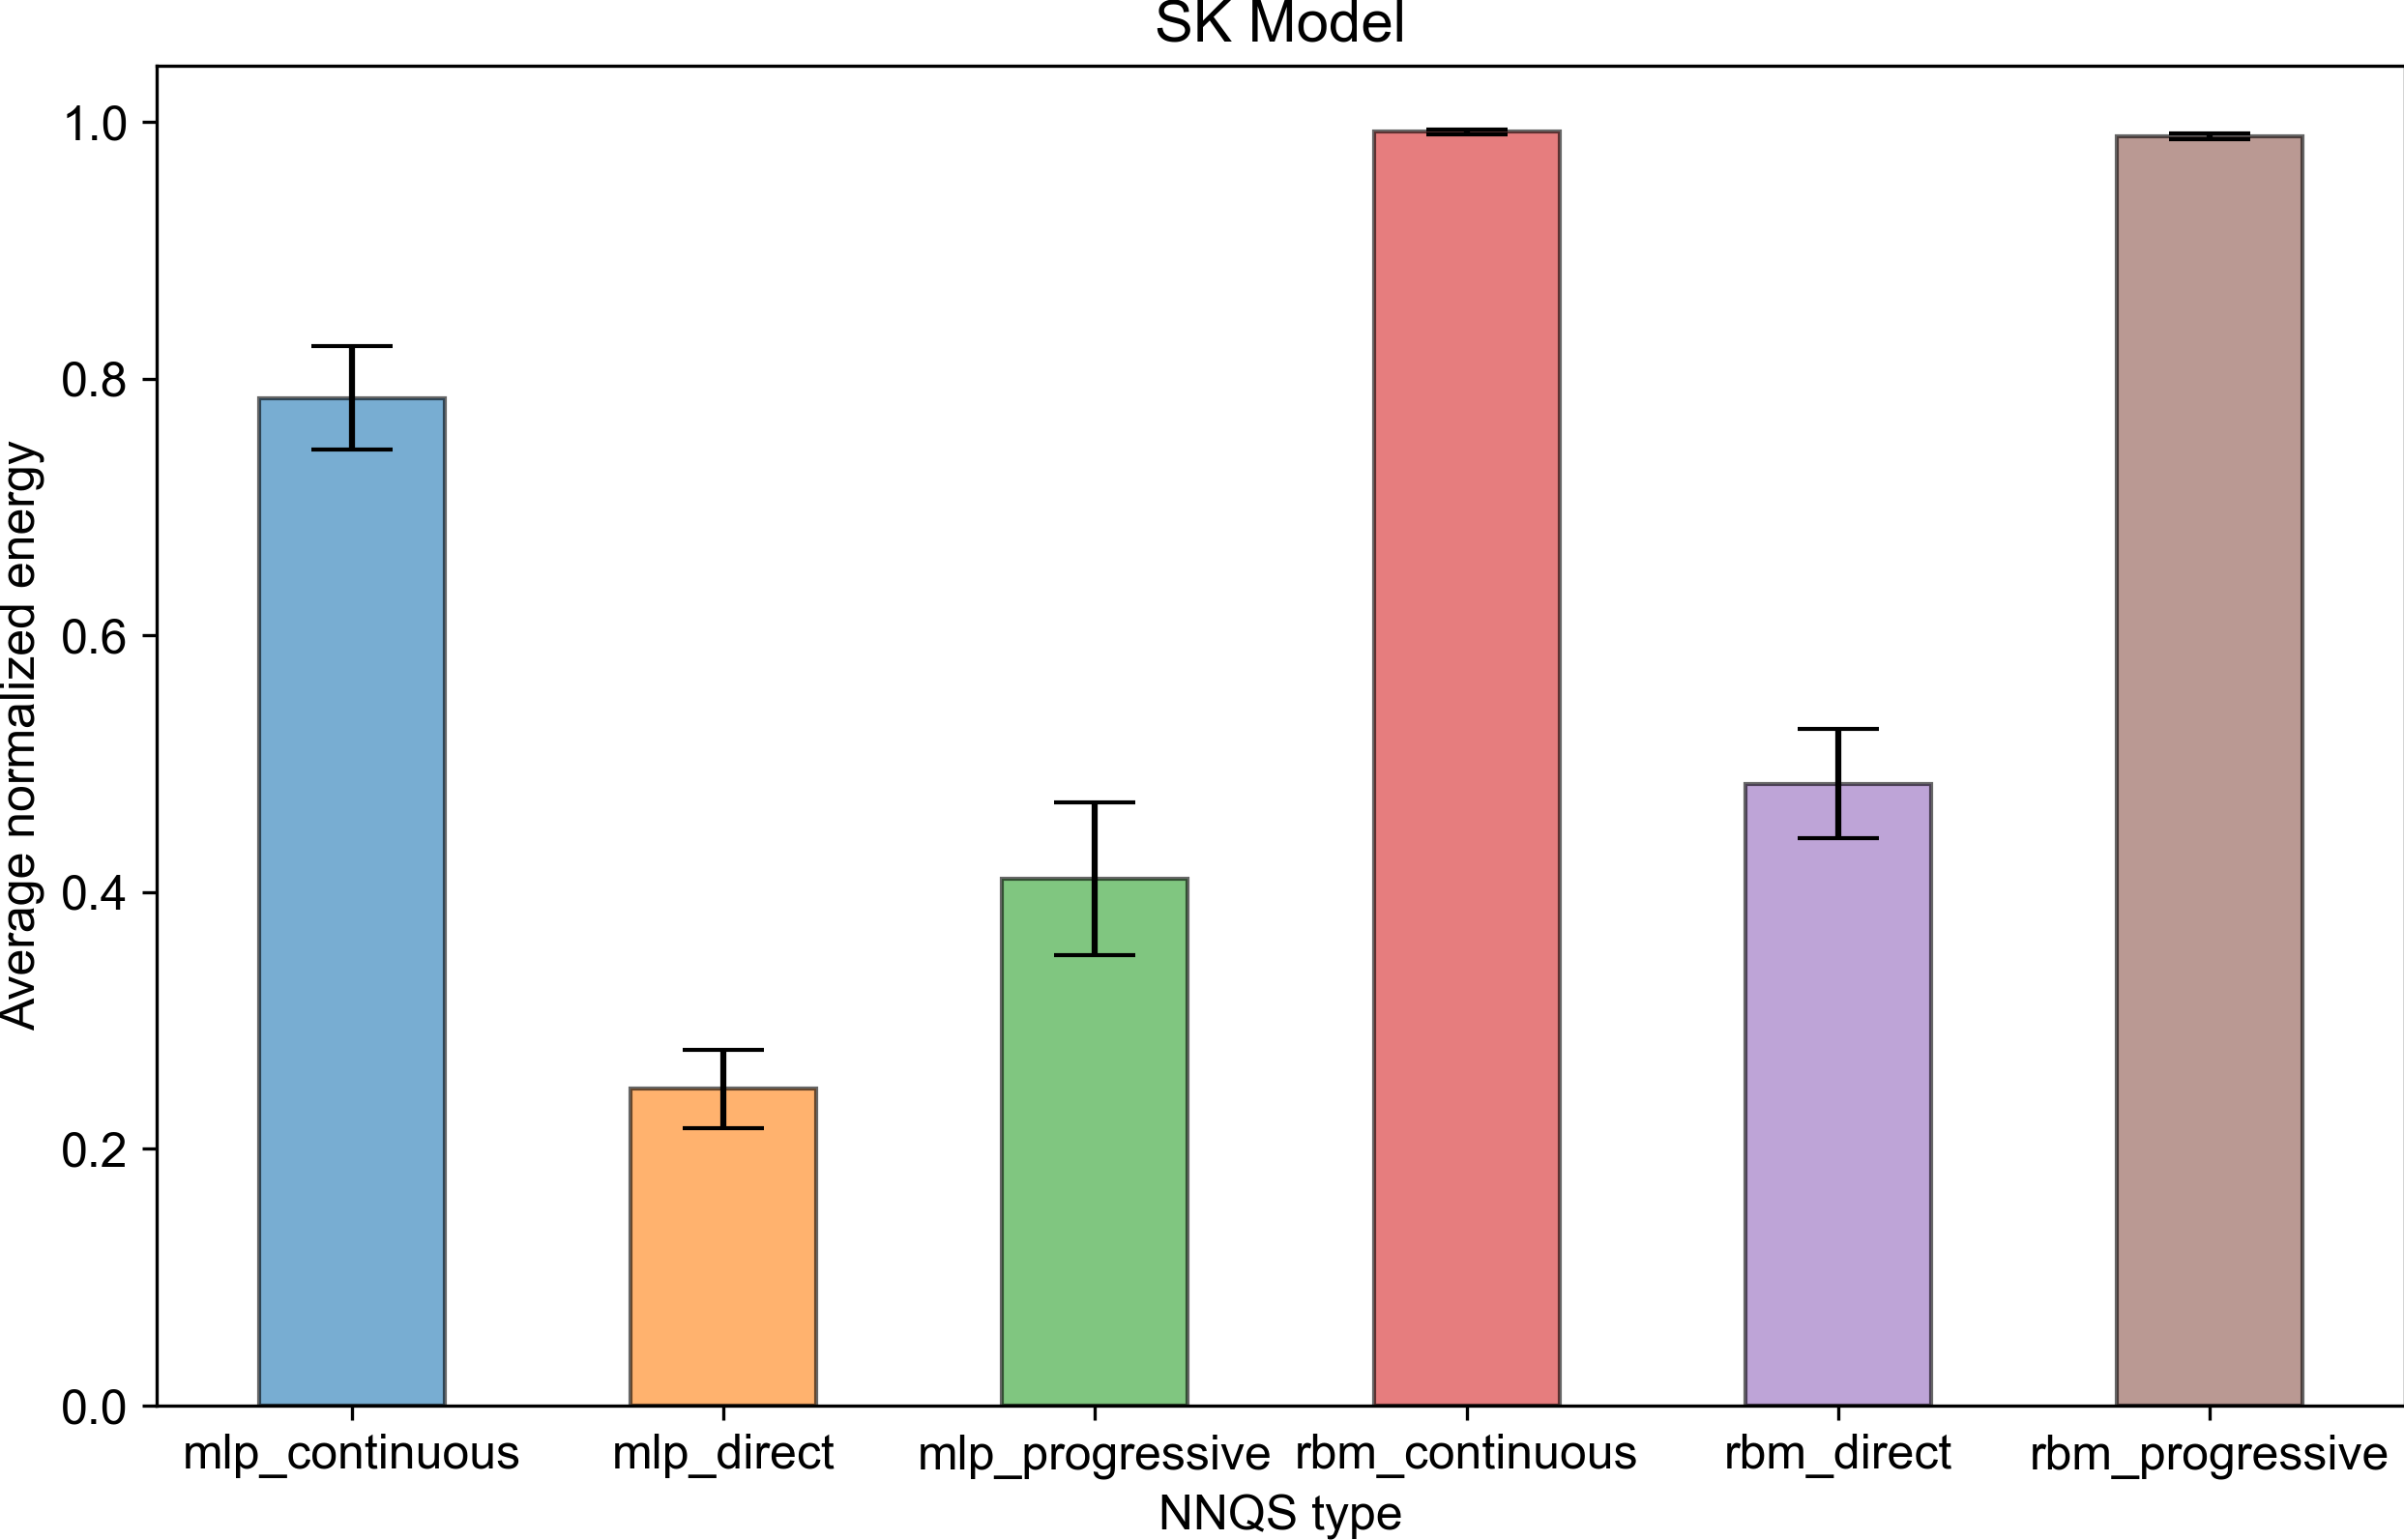
\includegraphics[width=0.49\textwidth]{images/skmodel_nnqs_avg.png}}\hfill
    \subfloat[Success probability]{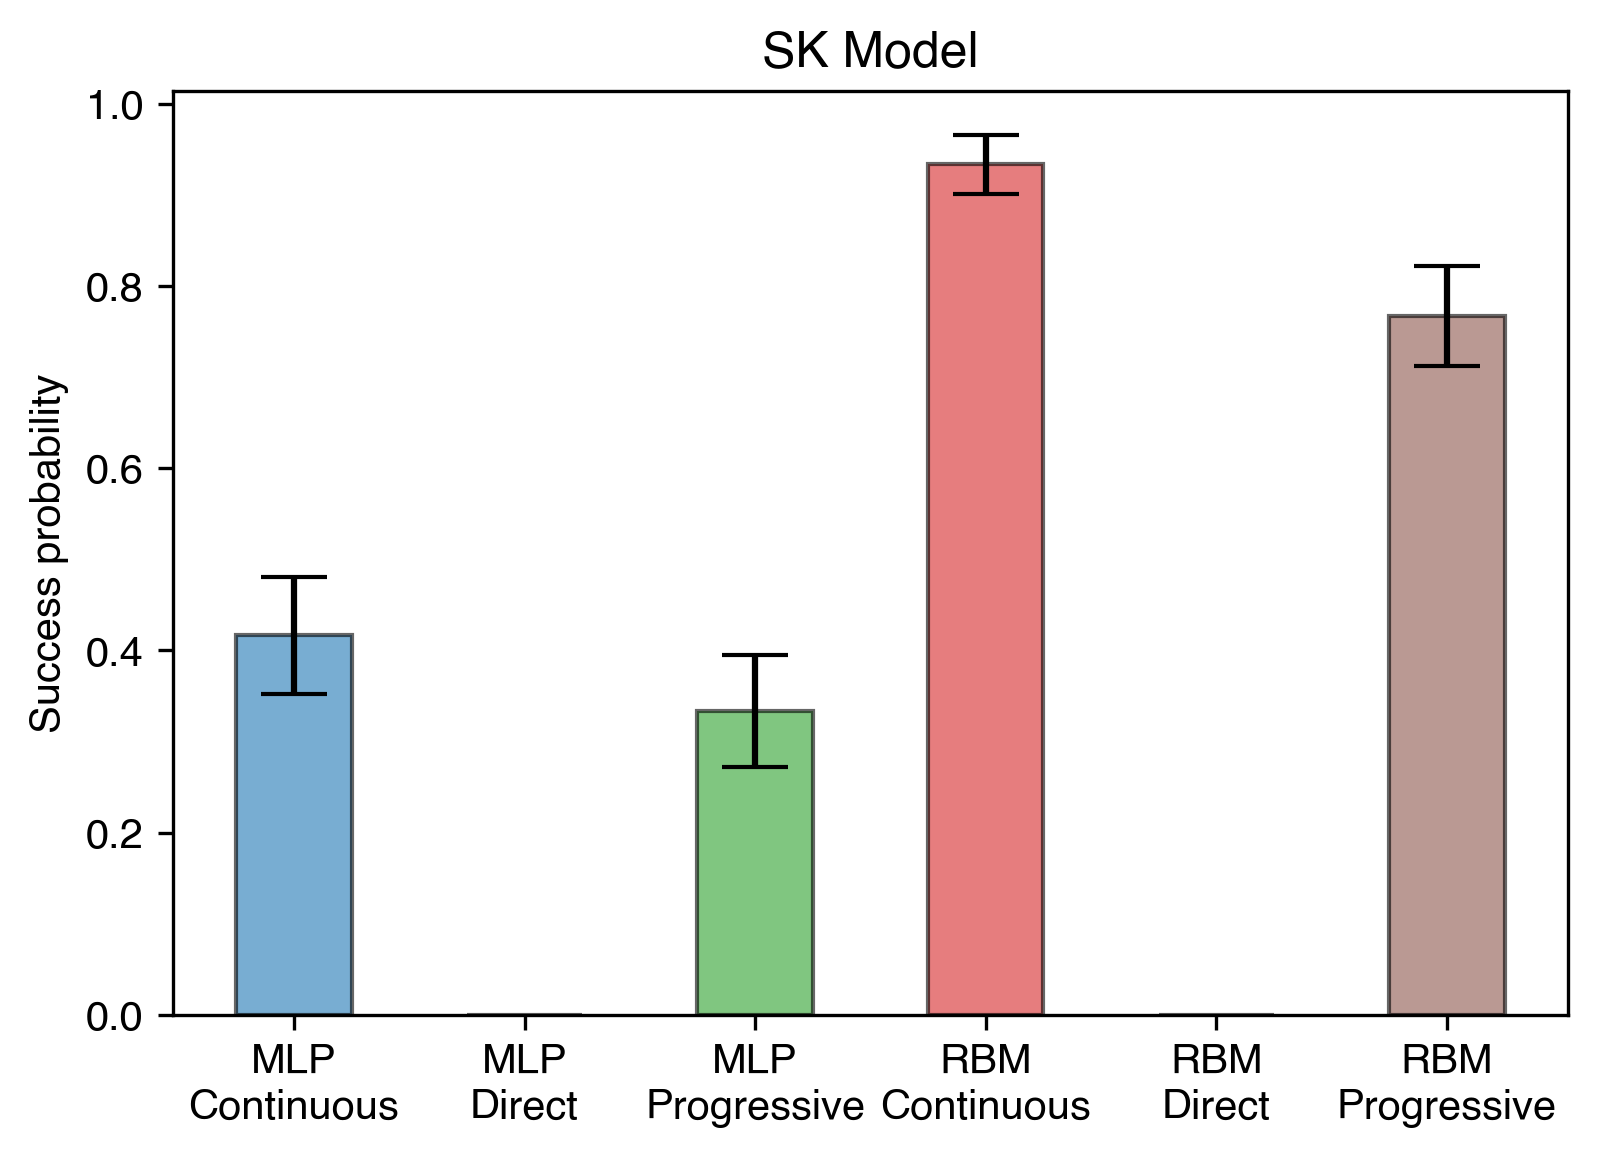
\includegraphics[width=0.49\textwidth]{images/skmodel_nnqs_success_avg.png}}
    \caption{Average performance of different NNQS types for SK model}
    \label{nnqs-skmodel-average}
\end{figure}

For the SK model dataset, the continuous training algorithm with the RBM generally performed the best in terms of normalized energy and success probability, shown in \autoref{nnqs-skmodel-size}. The performance averaged across all sizes, shown in \autoref{nnqs-skmodel-average}, also highlights that the RBM with a continuous training algorithm performs the best. However, it is interesting that the direct training schemes have poor performance with small problem sizes ($\leq 50$) but are relatively better at higher problem sizes ($100, 250$).

Across all the problem sets, we see that the RBM has a better average performance compared to the MLP in both average normalized energy and success probability for each training algorithm. In terms of training schemes, direct training performs the worst among the 3, and continuous training performs better than progressive training. Using the RBM with a continuous training scheme gives the highest normalized performance across all datasets.

\section{Future Work}
Future studies could investigate if more state-of-the-art machine learning models such as Graph Neural Networks or Attention-based Neural Networks can be used as the underlying architecture for NNQS.

To investigate whether the NNQS closely models the wave function of a D-wave solver in the annealing process, we can do a quench of the D-wave annealing process in order to take a snapshot of the intermediate state. Some initial work is detailed in \autoref{appendix:quenching} but is not included in the main report as the results are not substantial.